\documentclass[times,twocolumn,final]{elsarticle}
%DIF LATEXDIFF DIFFERENCE FILE
%DIF DEL source_01549.tex                            Sun Oct 11 14:07:30 2026
%DIF ADD Manuscript_conservative_submission_r2.tex   Sun Oct 11 14:07:30 2026

\usepackage{cag}
\usepackage{framed,multirow}
\usepackage{amssymb}
\usepackage{amsmath}
\usepackage{lineno}
\usepackage{graphicx}
\usepackage{booktabs}
%DIF 10d10
%DIF < \usepackage{placeins}
%DIF -------
\setcounter{totalnumber}{6}
\setcounter{topnumber}{4}
\setcounter{bottomnumber}{4}
\renewcommand{\topfraction}{0.92}
%DIF 15a14
\renewcommand{\dbltopfraction}{0.95} %DIF > 
%DIF -------
\renewcommand{\textfraction}{0.05}
\renewcommand{\floatpagefraction}{0.85}

%DIF 18-19d18
%DIF < \newtheorem{proposition}{Proposition}
%DIF < \newtheorem{remark}{Remark}
%DIF -------

\journal{Computers \& Graphics}
%DIF PREAMBLE EXTENSION ADDED BY LATEXDIFF
%DIF CFONT PREAMBLE %DIF PREAMBLE
\RequirePackage{color}\definecolor{RED}{rgb}{1,0,0}\definecolor{BLUE}{rgb}{0,0,1} %DIF PREAMBLE
\DeclareOldFontCommand{\sf}{\normalfont\sffamily}{\mathsf} %DIF PREAMBLE
\providecommand{\DIFadd}[1]{{\protect\color{blue} \sf #1}} %DIF PREAMBLE
\providecommand{\DIFdel}[1]{{\protect\color{red} \scriptsize #1}} %DIF PREAMBLE
%DIF SAFE PREAMBLE %DIF PREAMBLE
\providecommand{\DIFaddbegin}{} %DIF PREAMBLE
\providecommand{\DIFaddend}{} %DIF PREAMBLE
\providecommand{\DIFdelbegin}{} %DIF PREAMBLE
\providecommand{\DIFdelend}{} %DIF PREAMBLE
\providecommand{\DIFmodbegin}{} %DIF PREAMBLE
\providecommand{\DIFmodend}{} %DIF PREAMBLE
%DIF IDENTICAL PREAMBLE %DIF PREAMBLE
\providecommand{\DIFaddFL}[1]{\DIFadd{#1}} %DIF PREAMBLE
\providecommand{\DIFdelFL}[1]{\DIFdel{#1}} %DIF PREAMBLE
\providecommand{\DIFaddbeginFL}{\DIFaddbegin} %DIF PREAMBLE
\providecommand{\DIFaddendFL}{\DIFaddend} %DIF PREAMBLE
\providecommand{\DIFdelbeginFL}{\DIFdelbegin} %DIF PREAMBLE
\providecommand{\DIFdelendFL}{\DIFdelend} %DIF PREAMBLE
%DIF LISTINGS PREAMBLE %DIF PREAMBLE
\RequirePackage{listings} %DIF PREAMBLE
\RequirePackage{color} %DIF PREAMBLE
\lstdefinelanguage{DIFcode}{ %DIF PREAMBLE
%DIF DIFCODE_CFONT %DIF PREAMBLE
  moredelim=[il][\color{red}\scriptsize]{\%DIF\ <\ }, %DIF PREAMBLE
  moredelim=[il][\color{blue}\sffamily]{\%DIF\ >\ } %DIF PREAMBLE
} %DIF PREAMBLE
\lstdefinestyle{DIFverbatimstyle}{ %DIF PREAMBLE
	language=DIFcode, %DIF PREAMBLE
	basicstyle=\ttfamily, %DIF PREAMBLE
	columns=fullflexible, %DIF PREAMBLE
	keepspaces=true %DIF PREAMBLE
} %DIF PREAMBLE
\lstnewenvironment{DIFverbatim}{\lstset{style=DIFverbatimstyle}}{} %DIF PREAMBLE
\lstnewenvironment{DIFverbatim*}{\lstset{style=DIFverbatimstyle,showspaces=true}}{} %DIF PREAMBLE
%DIF END PREAMBLE EXTENSION ADDED BY LATEXDIFF

\renewcommand{\DIFaddbeginFL}{}
\renewcommand{\DIFaddendFL}{}
\renewcommand{\DIFdelbeginFL}{}
\renewcommand{\DIFdelendFL}{}
\renewcommand{\DIFaddFL}[1]{#1}
\renewcommand{\DIFdelFL}[1]{}
\setcounter{dbltopnumber}{3}
\renewcommand{\dbltopfraction}{0.90}
\renewcommand{\textfraction}{0.10}
\begin{document}

\begin{frontmatter}

\title{Timestep-Conditioned Adapter Scaling for Multi-view Diffusion Texture Generation}

% Double-anonymized review: author names, affiliations, and acknowledgements
% (including funding) are provided only on the separately uploaded title page.

\begin{abstract}
  \DIFaddbegin \DIFadd{Geometry-conditioned multi-view diffusion uses adapter strength to balance geometric alignment and generated appearance. We evaluate }\DIFaddend Timestep-Conditioned Adapter Scaling (TCAS), a training-free   \DIFaddbegin \DIFadd{temporal control on the existing GeoTex-Adapter residual path. In the original blinded study, }\DIFaddend C3   \DIFaddbegin \DIFadd{received 58.1\% of overall-quality choices (95\% cluster-bootstrap CI $[50.1,65.8]$}\DIFaddend ;   \DIFaddbegin \DIFadd{30 objects, 24 participants). On 300 input-disjoint Fresh C objects, C3 improves paired FG-PSNR over global Fixed Low (GFL) by $+0.52$ dB (95\% object-bootstrap CI $[+0.40,+0.64]$). Strong fixed and linear controls show that the measured advantage depends on comparator and endpoint; equal-budget Fixed Mean and Late-high exceed C3 on FG-PSNR. A ten-object calibrated bake pilot finds lower unseen-view FG-LPIPS for Late-high than Fixed Mean. A native fifty-object MV-Adapter test estimates a second-interface effect whose primary interval includes zero}\DIFaddend . These results   \DIFaddbegin \DIFadd{characterize temporal adapter control }\DIFaddend within the tested   \DIFaddbegin \DIFadd{texturing pipeline}\DIFaddend .
\end{abstract}

\begin{keyword}
\KWD
multi-view diffusion   \sep 3D   \DIFaddbegin \DIFadd{texturing }\DIFaddend \sep   \DIFaddbegin \DIFadd{geometry adapter }\DIFaddend \sep   \DIFaddbegin \DIFadd{residual }\DIFaddend scaling \sep   \DIFaddbegin \DIFadd{timestep conditioning
}\DIFaddend \end{keyword}

\end{frontmatter}

\linenumbers

\section{Introduction}
\label{sec:intro}

 
 \DIFaddbegin \DIFadd{Multi-view texture generation uses image diffusion to synthesize target views and then projects or bakes them onto an existing surface. Geometry adapters make normals, depth and foreground information available to the denoiser, but the strength of that information also affects surface appearance. An aggregate structural score alone cannot determine a useful setting: local variation may represent detail or unwanted patterns, }\DIFaddend and   \DIFaddbegin \DIFadd{image-space agreement must be considered alongside the final projected appearance}\DIFaddend .

 
 \DIFaddbegin \DIFadd{The 01549 study investigated this inference-control problem in an MVPainter-style pipeline through fixed-scale diagnostics, a 24-object comparison of 17 control variants, and a blinded preference study. TCAS applies a requested scale over denoising progress without training additional parameters or modifying the base model or adapter weights. Its recorded C3 profile, $(1.25,2.50,1.25)$, uses a stronger middle request and conservative early/late requests. This revision retains that method and development identity and evaluates the profile against stronger controls rather than searching for another C3 configuration.
}\DIFaddend 

  \DIFaddbegin \DIFadd{The central question is when a temporal control improves the tested outcome beyond an available fixed scale. We distinguish the requested multiplier, its applied value after native caps, and the resulting activation-dependent correction. A matched 300-object Fresh C evaluation supplies common-input paired comparisons; a same-cohort four-control budget match separates stage allocation from a larger applied-scale sum. Calibrated unseen-view baking and a native-camera MV-Adapter test extend the evidence to downstream appearance and a second conditioning interface. The original preference study remains a separate subjective evaluation of its own stimuli}\DIFaddend .

 
 \DIFaddbegin \DIFadd{Layer- and timestep-dependent scheduling is established prior work. Scheduled Style Injection (SSI) studies layer/time schedules and geometry-conditioned ControlNet strength scheduling. TCAS applies temporal control to the existing GeoTex residual path, whose normal, depth and foreground inputs, native layer caps, and activation-dependent corrections define a different intervention. The study contributes a controlled }\DIFaddend multi-view   \DIFaddbegin \DIFadd{texturing evaluation: the original preference result, a held-out paired comparison with strong controls, calibrated baking, and a native second-interface test}\DIFaddend .

The   \DIFaddbegin \DIFadd{contributions are}\DIFaddend :

(1)   \DIFaddbegin \DIFadd{\textbf{Executable inference-time control.} TCAS specifies a temporal scale on an existing geometry adapter, with explicit requested/applied semantics and no additional learned parameters. Historical fixed-scale and C3 development records explain the method's origin}\DIFaddend .

(2)   \DIFaddbegin \DIFadd{\textbf{Matched comparison with strong controls.} The 300-object Fresh C study reports paired gains, endpoint trade-offs and object-level variation. Its six-condition addendum combines four equal-applied-budget allocation controls with two strength controls, distinguishing the stage question from the C3--Fixed Low amplitude change (Table~\ref{tab:matched-budget300})}\DIFaddend .

(3)   \DIFaddbegin \DIFadd{\textbf{Preference and application evaluation.} The original blinded preference study supports an overall-quality preference for C3. Calibrated eleven-unseen-view baking on ten objects tests how generated results project into appearance and identifies the named Late-high--Fixed Mean LPIPS comparison (Tables~\ref{tab:preference} and \ref{tab:new-bake})}\DIFaddend .

(4)   \DIFaddbegin \DIFadd{\textbf{Native second-interface test.} A fifty-object MV-Adapter comparison evaluates the same stage-allocation question on a distinct geometry-conditioning interface and reports its complete seven-condition matrix (Table~\ref{tab:new-mva})}\DIFaddend .

\section{Related Work}
\label{sec:related}

\subsection{3D Texture Generation and Multi-view Diffusion}
\label{subsec:3dtex}

Single-image 3D generation is often decomposed into geometry generation and texture generation.   \DIFaddbegin \DIFadd{Single-image-to-3D}\DIFaddend , multi-view diffusion, and sparse-view reconstruction methods have   \DIFaddbegin \DIFadd{improved structural stability and view synthesis \cite{liu2023zero1to3,shi2023zero123pp,liu2023syncdreamer,long2023wonder3d,shi2024mvdream,wang2023imagedream,xu2024instantmesh,ke2024era3d}. Texture synthesis remains a distinct challenge for asset }\DIFaddend realism and usability   \DIFaddbegin \DIFadd{\cite{perla2026survey}. Many systems generate RGB views with }\DIFaddend 2D   \DIFaddbegin \DIFadd{diffusion and }\DIFaddend project or bake   \DIFaddbegin \DIFadd{them onto a }\DIFaddend surface \cite{chen2023text2tex,richardson2023texture,poole2023dreamfusion,chen2023fantasia3d}.   \DIFaddbegin \DIFadd{Recent work also explores }\DIFaddend exemplar-based texture synthesis   \DIFaddbegin \DIFadd{and }\DIFaddend diffusion-based procedural   \DIFaddbegin \DIFadd{materials \cite{guzman2026adaptive,lv2025interpretable}}\DIFaddend .

  Paint3D, MVPaint, Hunyuan3D 2.0, and MVPainter   \DIFaddbegin \DIFadd{use geometry-conditioned }\DIFaddend multi-view   \DIFaddbegin \DIFadd{generation in 3D texturing pipelines }\DIFaddend \cite{zeng2024paint3d,cheng2024mvpaint,lai2025hunyuan3d,shao2025mvpainter}. MV-Adapter  \DIFaddbegin \DIFadd{, MVDiffusion, and other }\DIFaddend synchronized multi-view   \DIFaddbegin \DIFadd{methods address consistency through different adapter and denoising designs \cite{huang2024mvadapter,tang2023mvdiffusion,liu2024synchronized,xu2026wondertex}. These systems establish the graphics context for this work. The present evidence does not compare final baked-texture quality across those systems}\DIFaddend .

  \DIFaddbegin \subsection{Adapter-Augmented Diffusion Models and Geometric Control}
\DIFaddend \label{subsec:adapter}

  \DIFaddbegin \DIFadd{ControlNet and }\DIFaddend T2I-Adapter   \DIFaddbegin \DIFadd{provide learned spatial-conditioning branches or feature injections, whose contribution can be weighted by an inference-time condition-strength scale \cite{mou2023t2iadapter,zhang2023controlnet}. They establish conditioning strength as a practical control, but their injected tensors and scaling sites do not share a numerical dose with GeoTex. The GeoTex-Adapter path in the 01549 study already exposes an inference-time residual scale and evaluates fixed requests. TCAS reuses that control point as a three-stage request over sampling progress, while recording how wrapper-group caps change the applied values and how adapter activations determine the resulting corrections. It adds no learned branch or schedule selector}\DIFaddend . IP-Adapter introduces image prompts through decoupled attention \cite{ye2023ipadapter}  \DIFaddbegin \DIFadd{; LoRA and related methods use scaled }\DIFaddend low-rank   updates \cite{hu2022lora,liu2024dora,zhang2023adalora}.
 
 

\subsection{Diffusion Guidance Scheduling and Timestep Control}
\label{subsec:guidance}

  \DIFaddbegin \DIFadd{Diffusion denoising is often discussed in terms of coarse-to-fine evolution, and prior work varies guidance strength over sampling progress to study quality, diversity, or fidelity \cite{ho2020ddpm,song2021ddim,ho2022cfg,castillo2023adaptive}. Limited-interval }\DIFaddend classifier-free   \DIFaddbegin \DIFadd{guidance is one example; it changes the combination of conditional and unconditional score predictions \cite{kynkanniemi2024limited}.
}\DIFaddend 

  \DIFaddbegin \DIFadd{SSI is the closest scheduling precedent. It varies StyleID's query-mixing parameter across decoder layers and denoising time, tests schedule direction and shape, and applies scheduling to a separate }\DIFaddend geometry-conditioned   \DIFaddbegin \DIFadd{ControlNet branch; its reported ControlNet scheduling gains over fixed conditioning are modest relative to its style-injection results \cite{kulkarni2026ssi}. This prior work already covers the general idea of layer/time scheduling and geometry-conditioning schedules. TCAS acts on the residual correction produced by GeoTex-Adapter from normal, depth, and foreground-mask conditions, with group-specific wrapper caps; it does not modulate StyleID attention mixing or add a ControlNet branch. The task, interface, and measured endpoints differ, so SSI does not imply the Fresh C paired estimates, the requested/applied/residual accounting, or the observed image- and color-agreement failures. These task-specific measurements are the empirical contribution; the scheduling concept itself is not claimed as new}\DIFaddend .

  \DIFaddbegin \subsection{Multi-view Adapter Interfaces}
\label{subsec:mvinterfaces}

\DIFadd{MV-Adapter uses a condition guider for camera or geometry maps together with decoupled spatial, multi-view, and optional image cross-attention layers \cite{huang2024mvadapter}. MVDiffusion uses correspondence-aware attention modules to connect pixels across views \cite{tang2023mvdiffusion}. These interfaces differ from the GeoTex-Adapter residual branch studied here. The native MV-Adapter test is reported within its own implementation and cohort; earlier exploratory interface panels remain separately identified in Supplementary Sections S12 and S17}\DIFaddend .

\section{Method}
\label{sec:method}

\subsection{Task Definition and Base Pipeline}
\label{subsec:task}

This paper builds on the MVPainter-style geometry-controlled multi-view texture generation framework \cite{shao2025mvpainter} and studies how the inference-time strength of geometric condition injection affects the generated results. Figure~\ref{fig:overview}   \DIFaddbegin \DIFadd{shows the TCAS control gate on the GeoTex-Adapter residual path: the requested scale is limited by the wrapper's group-specific cap before the residual is added to frozen UNet features}\DIFaddend . Given a single reference image and the corresponding 3D geometry, the base pipeline   generates RGB texture images from six target views and   \DIFaddbegin \DIFadd{can pass them to downstream }\DIFaddend projection or texture baking. \DIFaddbegin \DIFadd{Fresh C evaluates target-view images; the separate ten-object pilot evaluates calibrated unlit baked meshes. }\DIFaddend We do not modify the base UNet, VAE, or pretrained adapter weights.
  

\begin{figure*}[t]
\centering
  \DIFaddbeginFL 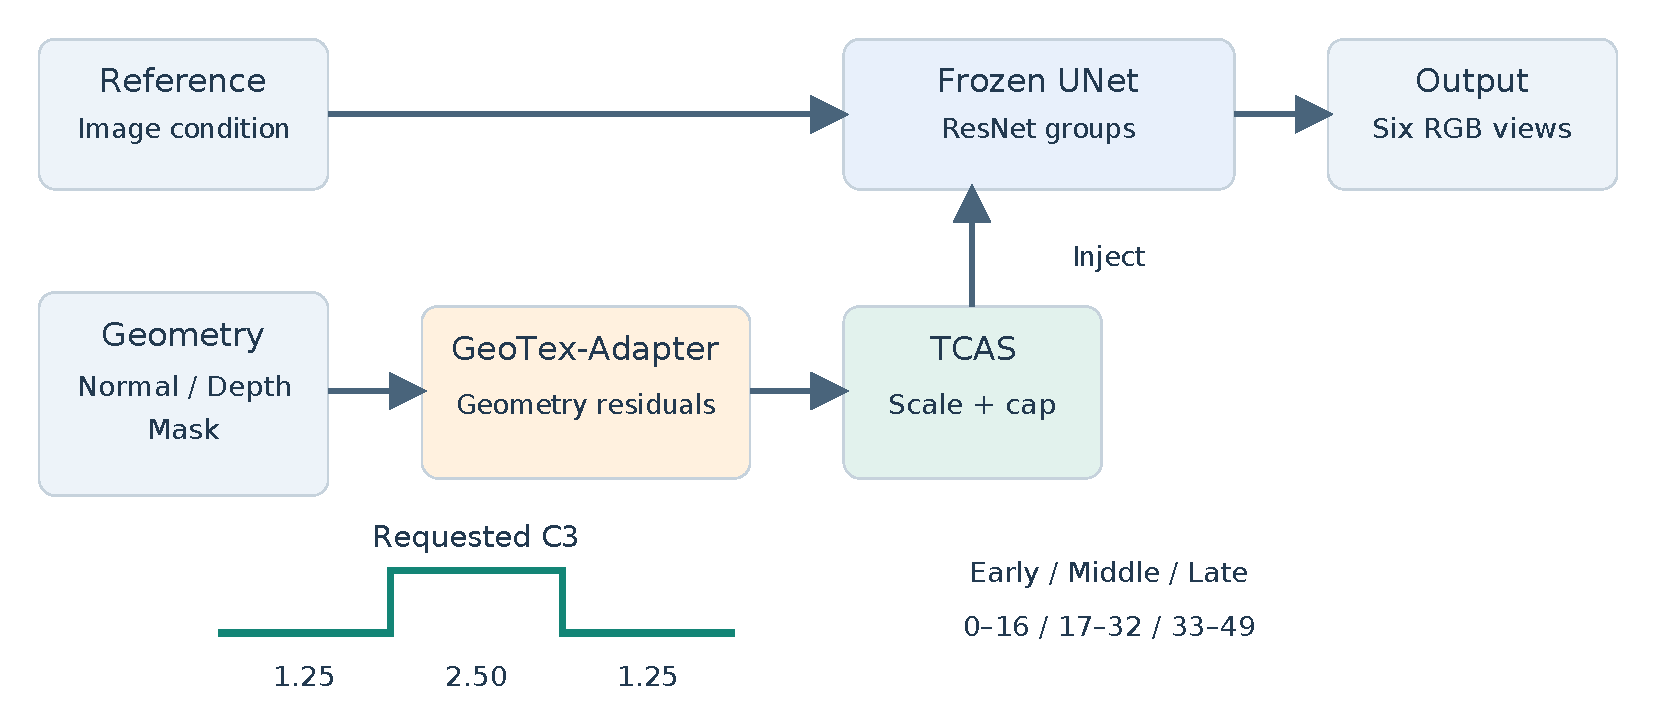
\includegraphics[width=\textwidth]{figures/fig1_tcas_control.pdf}
\caption{TCAS on the existing GeoTex residual path. Reference conditioning and five-channel geometry conditioning enter separate paths. The requested scale is capped per layer group before injection into the frozen UNet. The diagram abstracts multiple ResNet sites; steps are zero-based, and Fresh C shallow requests are capped at 0.8. This is an implementation schematic, not an experimental result.}
\DIFaddendFL \label{fig:overview}
\end{figure*}

During multi-view diffusion, the 3D geometry is rendered into normal maps, depth maps, and foreground masks, denoted as:
\begin{equation}
\mathbf{G} = \{G_\text{normal}, G_\text{depth}, G_\text{mask}\}.
\end{equation}

The geometric adapter maps these conditions to a residual correction term and injects it into the intermediate hidden states of the UNet. For   \DIFaddbegin \DIFadd{inference step $j$ with normalized execution progress $p_j$}\DIFaddend , the adapter injection can be written as:
  \DIFaddbegin \begin{equation}
\mathbf{h}'_{j,\ell} = \mathbf{h}_{j,\ell} + s_{\mathrm{app}}(p_j,\ell)\, A^\ell_\phi(\mathbf{h}_{j,\ell}, \mathbf{G}),
\label{eq:injection}
\end{equation}\DIFaddend 
  \DIFaddbegin \DIFadd{Here $\ell$ indexes an injected layer group. The \emph{requested scale} $s_{\mathrm{req}}(p_j,\ell)$ is the value assigned by the profile; the \emph{applied scale} is the value used by the wrapper,
}\begin{equation}
s_{\mathrm{app}}(p_j,\ell)=\min\!\bigl(s_{\mathrm{req}}(p_j,\ell),c_\ell\bigr),
\end{equation}
\DIFadd{when the native cap $c_\ell$ is active, and otherwise equals the request. The resulting correction is $\mathbf{r}_{j,\ell}=s_{\mathrm{app}}(p_j,\ell)A^\ell_\phi(\mathbf{h}_{j,\ell},\mathbf{G})$; its \emph{post-scale residual magnitude} is $m_{j,\ell}=\|\mathbf{r}_{j,\ell}\|_2$. Thus neither a requested nor an applied scale label alone determines the correction magnitude.
}

\DIFadd{In the audited Fresh C wrapper, }\DIFaddend the   \DIFaddbegin \DIFadd{three cap groups map the GeoTex residual wrappers on the UNet ResNet blocks as follows: deep comprises the UNet middle block and $\texttt{up\_0}$, middle is $\texttt{up\_1}$, and shallow is $\texttt{up\_2}$. These names identify the implementation's grouped injection points; they do not assert universal semantic roles for denoising stages. The corresponding Fresh C caps are 3.0, 3.5, and 0.8. C3's shallow request of 1.25 is therefore applied as 0.8, while its deep and middle requests pass unchanged. GFL and GFH also clip at the shallow cap. These equations and caps describe the explicitly requested-scale path. The unset-scale GeoTex wrapper bypasses this cap operation and is a distinct path; its generated outputs are not available here (Supplementary Section S20). These cap values describe the audited Fresh C wrapper; row-level cap semantics for the historical 24-object probe are not fully recoverable. TCAS scales a geometry }\DIFaddend residual added to   \DIFaddbegin \DIFadd{feature activations; it does not reweight conditional and unconditional score predictions as classifier-free guidance does.
}\DIFaddend 

  \DIFaddbegin \subsection{Image-Space Metrics and Texture-Variation Diagnostics}
\DIFaddend \label{subsec:metrics}

  \DIFaddbegin \DIFadd{We use separate terms for separate outcomes. \emph{Image-space agreement} refers to target-view PSNR, LPIPS, and SSIM measurements on the named image regions; it is not a measure of final 3D material quality. \emph{Reference-color agreement} refers to color differences such as CIEDE2000 computed against the corresponding reference. \emph{Texture variation} refers to statistics such as RGB standard deviation, Laplacian variance, gradient magnitude, and high-frequency energy; these may rise with detail or artifacts and are not fidelity measures. \emph{Subjective preference} refers only to the submitted forced-choice study. \emph{Baked 3D appearance} refers to rendered mesh outputs after texture projection or baking, while \emph{PBR/material fidelity} additionally concerns appearance under the material and illumination model. These endpoints are not interchangeable. }\DIFaddend FG-SSIM, Edge-SSIM, and Crop-SSIM   \DIFaddbegin \DIFadd{quantify structural similarity on the indicated image regions; PSNR measures pixel error; LPIPS compares learned image features \cite{wang2004ssim,zhang2018lpips}.
}

\DIFaddend Laplacian variance, RGB standard deviation, and gradient magnitude   \DIFaddbegin \DIFadd{can describe local }\DIFaddend high-frequency  
 \DIFaddbegin \DIFadd{or color variation. For example, a foreground Laplacian statistic may be written as
}\begin{equation}
M_{\mathrm{var}}=\operatorname{Var}\!\left(\operatorname{Lap}(I_{\mathrm{out}}\odot G_{\mathrm{mask}})\right),
\end{equation}\DIFaddend 
where   \DIFaddbegin \DIFadd{$G_{\mathrm{mask}}$ is }\DIFaddend the foreground mask  . A larger   \DIFaddbegin \DIFadd{value is not necessarily better: detail, noise, repeated patterns, or artifacts can all increase local variation. We therefore do not interpret these proxies as texture fidelity or use them alone to claim that a schedule better preserves reference appearance}\DIFaddend .

  \DIFaddbegin \subsection{TCAS Control Semantics and Comparison Design}
\DIFaddend \label{subsec:tcas}

  \DIFaddbegin \DIFadd{TCAS }\DIFaddend replaces a globally fixed \DIFaddbegin \DIFadd{requested }\DIFaddend adapter scale with a   \DIFaddbegin \DIFadd{piecewise profile over normalized sampling progress. The early/middle/late partition is an operational description, not a universal claim about the function of every denoising stage. C3's low--high--low profile is the specific development choice evaluated in this revision; it is not presented as an independently derived optimum}\DIFaddend .

To avoid ambiguity caused by different raw timestep directions in different schedulers,   \DIFaddbegin \DIFadd{$p_j=j/(T-1)$ denotes execution progress for inference step $j\in\{0,\ldots,T-1\}$. Thus $p=0$ is the first update from }\DIFaddend the   \DIFaddbegin \DIFadd{initial noisy latent and $p=1$ is the last denoising update before decoding. For $T=50$, TCAS divides execution into steps 0--16, 17--32, and 33--49 (17/16/17 steps):
}\begin{equation}
s_{\mathrm{req}}(p) = \begin{cases} s_e, & 0 \leq p < 1/3 \\ s_m, & 1/3 \leq p < 2/3 \\ s_l, & 2/3 \leq p \leq 1 \end{cases}.
\label{eq:tcas}
\end{equation}\DIFaddend 

\DIFaddbegin \DIFadd{We call this variation across the 50 inference steps the \emph{temporal allocation}. A \emph{layer allocation} varies the requested scale across the three wrapper groups at a fixed step. For a schedule with applied values $s_{\mathrm{app}}(j,\ell)$, its per-group applied-scale sum is $B_\ell=\sum_j s_{\mathrm{app}}(j,\ell)$; the unweighted sum $B_{\mathrm{nom}}=\sum_\ell B_\ell$ is a \emph{nominal applied-scale budget}. It does not weight scales by adapter activations. We log post-scale correction summaries, including wrapper-level $L_2$ norm and mean absolute entry. The three wrapper groups operate on feature maps with different spatial dimensions, and the traces do not retain channel counts; raw $L_2$ values are therefore not used for cross-layer dose comparisons. The per-entry mean absolute correction reported in Supplementary Section~S4 is a dimension-normalized descriptive summary, not an equal-dose intervention. Correction magnitudes also depend on the current hidden state and earlier denoising updates, so equal nominal budgets do not imply equal realized corrections.
}

\DIFaddend The selected C3 configuration used in this paper is:
\begin{equation}
(s_e, s_m, s_l) = (1.25, 2.50, 1.25).
\end{equation}

  \DIFaddbegin \DIFadd{The low--high--low profile is a concrete inference-time intervention motivated by the submitted development analysis. Its stage interpretation is a task-specific hypothesis: the tested early, middle, and late allocations may produce different responses. Fresh C evaluates the recorded profile against matched controls but does not prove a universal function for any stage. TCAS adds no trained }\DIFaddend parameters and does not modify   \DIFaddbegin \DIFadd{base-model }\DIFaddend or adapter weights; it   \DIFaddbegin \DIFadd{replaces the requested scale during inference}\DIFaddend .

  \DIFaddbegin \paragraph{What C3 changes and what its comparisons identify}
\DIFadd{C3 requests 1.25 during steps 0--16, 2.50 during steps 17--32, }\DIFaddend and   \DIFaddbegin \DIFadd{1.25 during steps 33--49, applying that temporal profile to each of the three layer groups before native caps. In Fresh C, the applied deep and middle profiles retain those values; the shallow profile is clipped to 0.8 throughout. GFL requests 1.25 at every step and group, so its deep and middle values are 1.25 throughout and its shallow value is also clipped to 0.8. Their per-group applied-scale sums are therefore 82.5 versus 62.5 in deep and middle, and 40 for both in shallow. The C3--GFL contrast changes the middle-third deep/middle scale magnitude as well as its temporal allocation; it is not a timing-only comparison.
}\DIFaddend 

  \DIFaddbegin \DIFadd{To identify a temporal-placement contrast, controls must hold the per-layer applied values and nominal per-group sums fixed while moving the same values between time windows. To identify a scale-strength contrast, controls must hold the layer and temporal allocations fixed while changing amplitude. Both contrasts also require reporting post-scale correction summaries: matching requested values or applied-scale sums does not match the evolving residual corrections. Raw $L_2$ values are dimension-sensitive across wrapper groups and cannot establish cross-layer dose matching. The current 300-object allocation comparison exactly matches the applied sums in each layer group. This controls the scalar budget for }\DIFaddend the  
 \DIFaddbegin \DIFadd{total allocation effect, although it does not identify a residual-dose-independent mechanism. Post-hoc adjustment for state-dependent corrections cannot by itself recover that mechanism. The older strict-276 analysis is reported separately.
}\DIFaddend 

  \DIFaddbegin \paragraph{Development origin and scope of C3}
\DIFadd{The submitted 01549 paper records }\DIFaddend C3  
 \DIFaddbegin \DIFadd{$=(1.25,2.50,1.25)$ as the selected profile from a 24-object development probe containing 17 uniform, layer-wise, and time-conditioned variants. We retain this history to explain the profile evaluated here. Fresh C carries }\DIFaddend C3  

 \DIFaddbegin \DIFadd{forward without further schedule search; the profile is treated as an empirical candidate rather than }\DIFaddend a   \DIFaddbegin \DIFadd{derived optimum. Historical selection records and their evidence scope are detailed in Supplementary Section S10}\DIFaddend .

\DIFaddbegin \subsection{Geometry Adapter and Inference Interface}
\label{subsec:adapterimpl}

\DIFaddend GeoTex-Adapter is   \DIFaddbegin \DIFadd{treated as the fixed geometry-residual backbone, not as a new contribution of this paper}\DIFaddend . It receives a   \DIFaddbegin \DIFadd{five-channel input comprising a three-channel }\DIFaddend normal map, a   \DIFaddbegin \DIFadd{one-channel }\DIFaddend depth map, and a   \DIFaddbegin \DIFadd{one-channel }\DIFaddend foreground mask. A multi-scale   \DIFaddbegin \DIFadd{encoder produces residual features that }\DIFaddend are injected into   \DIFaddbegin \DIFadd{the frozen }\DIFaddend UNet. TCAS acts on the   \DIFaddbegin \DIFadd{requested multiplier along denoising progress; it does not retrain the adapter, the UNet, or the VAE and introduces no learned parameters}\DIFaddend .

  \DIFaddbegin \DIFadd{The first-round 01549 revision also reported a learned }\DIFaddend Full Adaptive Correction (FAC)  
 \DIFaddbegin \DIFadd{extension. We retain its controlled negative re-examination as a previously reported auxiliary result in Section~\ref{subsec:facreported} and Supplementary Table~S16; it is not a new 1008 training run. TCAS remains the paper's sole training-free method}\DIFaddend .

\section{Experiments}
\label{sec:experiments}

\subsection{Experimental Setup}
\label{subsec:setup}

\subsubsection{Experimental protocol and comparisons}

  \DIFaddbegin \DIFadd{The original 01549 study reports fixed-scale experiments, a 24-object schedule-development probe, and a pooled 300-object evaluation. These records motivate the present question and retain their historical identities. Current matched image-space estimates come from Fresh C, a separate 300-object UID-disjoint study; the cohort roles and provenance are summarized in Table~\ref{tab:cohort-map} and Supplementary Sections S8--S10}\DIFaddend .

  \DIFaddbegin \DIFadd{Fresh C is a matched image-space study on 300 frozen object identifiers, disjoint from the original }\DIFaddend 24-object   \DIFaddbegin \DIFadd{development probe, the original evaluation cohort, and the 1,118-object training list. Its primary run (No Adapter, GFL, GFH, C3) and same-cohort Generic Linear/LLH addendum share one frozen checkpoint, runner, inputs, target views, metric implementation, and seed policy. The registered primary endpoint is paired C3--GFL FG-PSNR. All six views are generated under the same object-level seed; condition-level records and checkpoint/run identities are listed in Supplementary Section S8. Other historical and retrospective cohorts are reported separately and are not pooled with Fresh C.
}\DIFaddend 

  \DIFaddbegin \begin{table*}[t]\centering\scriptsize
\caption{Evidence cohorts used for current conclusions. Historical development, preference and FAC records retain their original identities and are not pooled with these rows.}
\label{tab:cohort-map}
\begin{tabular}{llll}
\toprule \DIFaddFL{Cohort }& \DIFaddFL{Objects / controls }& \DIFaddFL{Evaluation domain }& \DIFaddFL{Role }\\
\midrule
\DIFaddFL{Fresh C primary + addendum }& \DIFaddFL{300 / 6 }& \DIFaddFL{GeoTex target images }& \DIFaddFL{UID-disjoint matched checkpoint comparison }\\
\DIFaddFL{Equal-budget addendum }& \DIFaddFL{Same 300 / 6 }& \DIFaddFL{GeoTex target images }& \DIFaddFL{Post-inspection allocation comparison }\\
\DIFaddFL{New native MV-Adapter }& \DIFaddFL{50 / 7 }& \DIFaddFL{Native-camera albedo targets }& \DIFaddFL{Internally frozen second-interface test }\\
\DIFaddFL{New bake pilot }& \DIFaddFL{10 / 7 + GT }& \DIFaddFL{Eleven unseen views per object }& \DIFaddFL{Input-compatible pilot; image outcomes previously known }\\
\DIFaddFL{Corrected earlier bake }& \DIFaddFL{Separate 5 }& \DIFaddFL{Unlit unseen views }& \DIFaddFL{Descriptive; supersedes erroneous estimates }\\
\bottomrule\end{tabular}
\end{table*}
\DIFaddend 

\subsubsection{Evaluation sets and metrics}

  \DIFaddbegin \DIFadd{The submitted paper also reports }\DIFaddend a 50-object   \DIFaddbegin \DIFadd{scale sweep, a purposive }\DIFaddend 26-object texture audit  \DIFaddbegin \DIFadd{, }\DIFaddend and   the 24-object  
 \DIFaddbegin \DIFadd{development probe. The sweep and probe remain historical context; the texture audit is retained as a selected diagnostic with its scope stated in Supplementary Sections S7 and S13. Fresh C reports foreground PSNR, LPIPS, SSIM, and }\DIFaddend Edge-SSIM   \DIFaddbegin \DIFadd{for target-view image agreement. The original 01549 preference study measures choices for its own stimuli. }\DIFaddend Laplacian variance, RGB standard deviation, and gradient magnitude  
 \DIFaddbegin \DIFadd{describe local variation, not fidelity or material quality}\DIFaddend .

\subsubsection{Implementation and dataset details}

 
 \DIFaddbegin \DIFadd{Fresh C uses one controlled-retraining GeoTex-Adapter checkpoint with the }\DIFaddend MVPainter-style   \DIFaddbegin \DIFadd{joint }\DIFaddend six-view   \DIFaddbegin \DIFadd{latent UNet and VAE, EulerDiscreteScheduler for }\DIFaddend 50   \DIFaddbegin \DIFadd{steps, and six fixed target views at 256$\times$256. Each object uses seed $42+\texttt{object\_idx}$ shared across conditions. Checkpoint identity, run manifests, cohort hashes, and historical checkpoint distinctions are recorded in Supplementary Section S8}\DIFaddend .

  \DIFaddbegin \DIFadd{Fresh C's native wrapper caps are deep 3.0, middle 3.5, and shallow 0.8. The recorded scale request, applied value, and post-scale residual norm are separate fields. The requested C3 profile is $(1.25,2.50,1.25)$; its shallow value is clipped to 0.8 in this run. The Generic Linear and LLH addendum conditions are separately defined and do not equalize realized residual dose. Detailed step- and layer-group records are supplied in the Supplement.
}

\DIFadd{The frozen evaluator computes FG-PSNR, FG-LPIPS, FG-SSIM, and }\DIFaddend Edge-SSIM   \DIFaddbegin \DIFadd{once on each full 3$\times$2 six-view composite. The primary comparison is C3--GFL FG-PSNR; secondary and addendum tests follow the stated families in Supplementary Section S2. Display-view scores are used only to check illustrated cases and do not replace the composite-level analysis}\DIFaddend .

\paragraph{Statistical reporting}
  \DIFaddbegin \DIFadd{Fresh C reports the object-level paired mean difference and percentile-bootstrap }\DIFaddend 95\%   \DIFaddbegin \DIFadd{interval from }\DIFaddend 10{,}000   \DIFaddbegin \DIFadd{object resamples. The registered primary C3--GFL FG-PSNR contrast is unadjusted as the single primary endpoint. Secondary and addendum families and their multiplicity adjustments are detailed in Supplementary Section S2. CIs outside that prespecified family are pointwise and descriptive. The earlier three-condition 3AFC study is reported separately below as a subjective preference result; it is not a Fresh C endpoint or evidence of texture fidelity}\DIFaddend .

  \DIFaddbegin \subsection{Historical Fixed-Scale Image-Space Diagnostics}
\DIFaddend \label{subsec:tradeoff}

Table~\ref{tab:sweep}   \DIFaddbegin \DIFadd{reproduces the }\DIFaddend 13-scale   \DIFaddbegin \DIFadd{sweep reported in the submitted 01549 manuscript. We retain it to preserve the original development question, but the object-level outputs, full run manifest, and metric implementation mapping are not available in the current authority. Its values and Figures~\ref{fig:curve}--\ref{fig:heatmap} are therefore historical diagnostics, not a new reanalysis or confirmatory evidence}\DIFaddend .

\begin{table}[t]
\centering
  \DIFaddbeginFL \caption{Historical 01549 report of a 13-scale sweep on the stated 50-object set. Values are reproduced from the submission and have not been independently recomputed from row-level outputs; they are retained as development diagnostics.}
\DIFaddendFL \label{tab:sweep}
\small
\begin{tabular}{lcccc}
\toprule
Scale & $\Delta$FG-SSIM$\uparrow$ & POS & $\Delta$Crop-SSIM$\uparrow$ & $\Delta$PSNR$\uparrow$ \\
\midrule
0.75 & $-$0.013 & 20/50 & +0.113 & 7.53 \\
0.90 & +0.024 & 30/50 & +0.137 & 8.32 \\
1.00 & +0.047 & 34/50 & +0.147 & 8.79 \\
1.10 & +0.070 & 36/50 & +0.159 & 9.08 \\
1.15 & +0.071 & 36/50 & +0.157 & 9.25 \\
1.25 & +0.088 & 37/50 & +0.161 & 9.37 \\
1.35 & +0.100 & 39/50 & +0.163 & 9.63 \\
1.50 & +0.113 & 40/50 & +0.163 & 9.76 \\
1.60 & +0.120 & 42/50 & +0.166 & 9.83 \\
1.75 & +0.127 & 43/50 & +0.173 & 9.97 \\
2.00 & +0.134 & 44/50 & +0.169 & 9.96 \\
2.25 & +0.142 & 43/50 & +0.175 & 9.91 \\
2.50 & +0.145 & 44/50 & +0.165 & 9.91 \\
\bottomrule
\end{tabular}
\end{table}

  \DIFaddbegin \DIFadd{The submitted table reports a rising }\DIFaddend $\Delta$FG-SSIM   \DIFaddbegin \DIFadd{over most of the listed scale range and a near-plateau in the crop metric at higher settings. We retain this reported pattern only as historical motivation: absent row-level outputs and a complete run manifest, we do not treat it as an independently confirmed scale-response law. It motivates asking whether a single aggregate structural score fully describes the effect of adapter scaling.
}\DIFaddend 

\begin{figure}[t]
\centering
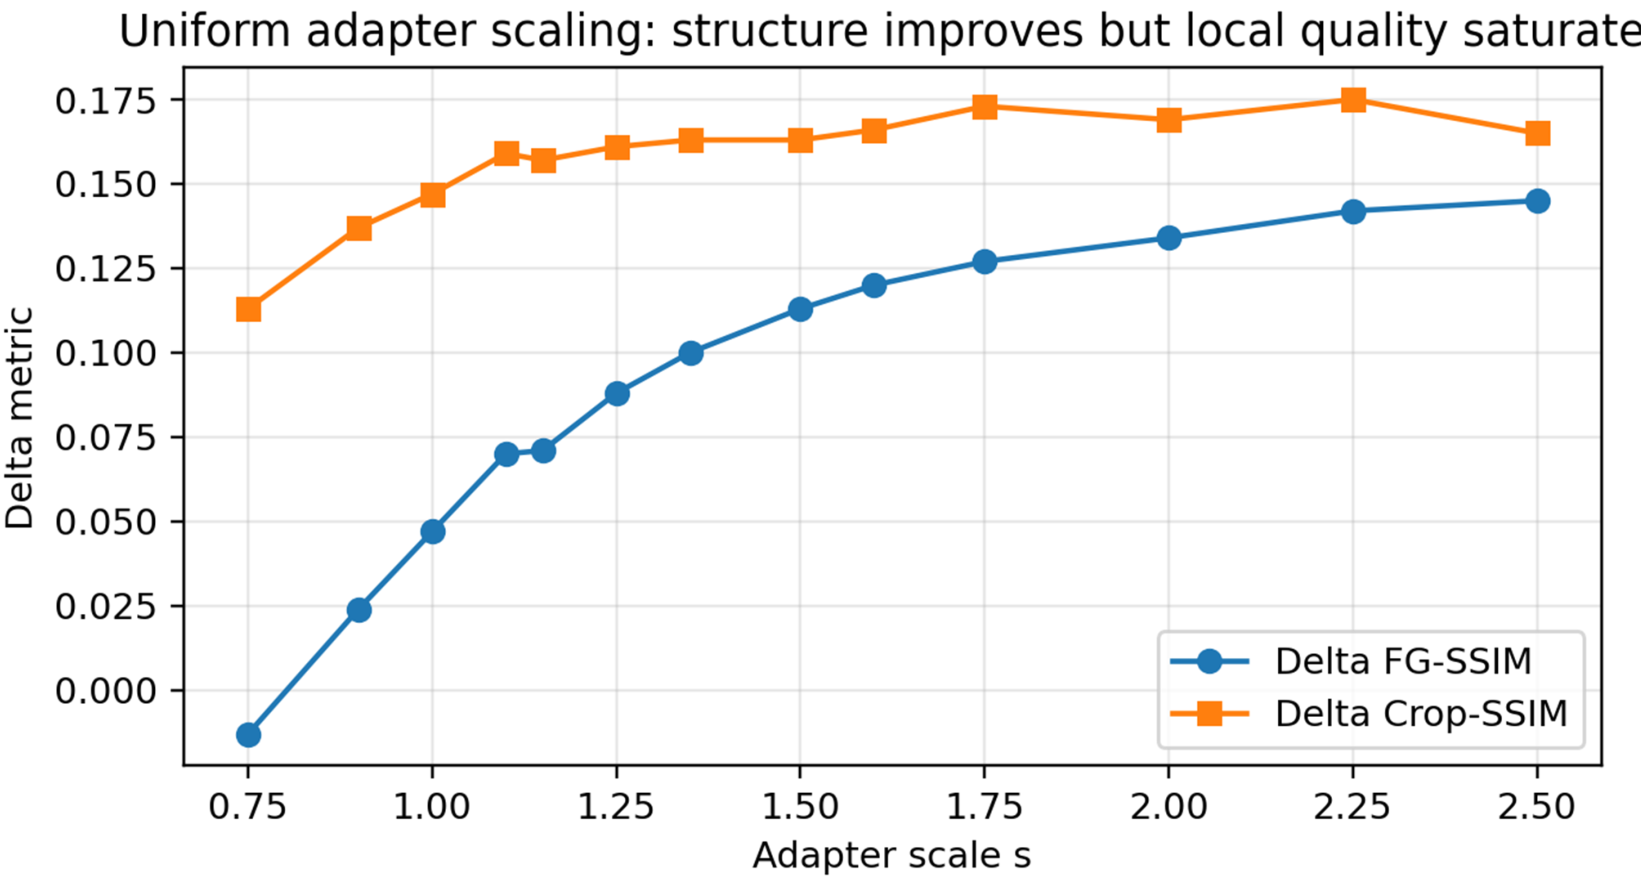
\includegraphics[width=\columnwidth]{fig2.pdf}
  \DIFaddbeginFL \caption{Historical fixed-scale diagnostic from the submitted 01549 paper. The plotted source reports FG-SSIM and Crop-SSIM over adapter scales; the underlying object-level run records are not available for independent reanalysis. It motivates measuring more than one endpoint, but is not a current confirmatory result.}
\DIFaddendFL \label{fig:curve}
\end{figure}

  \DIFaddbegin \DIFadd{The submitted heatmap depicts }\DIFaddend object-level  


 \DIFaddbegin \DIFadd{variation across the reported scales, but its underlying rows cannot be reconstructed from the current evidence archive. We retain the visual diagnostic as part of the 01549 research history and do not infer a population-level response distribution from it}\DIFaddend .  

 \DIFaddbegin \DIFadd{The updated Fresh C analysis below uses its own frozen cohort and matched inputs}\DIFaddend .

\begin{figure}[t]
\centering
  \DIFaddbeginFL 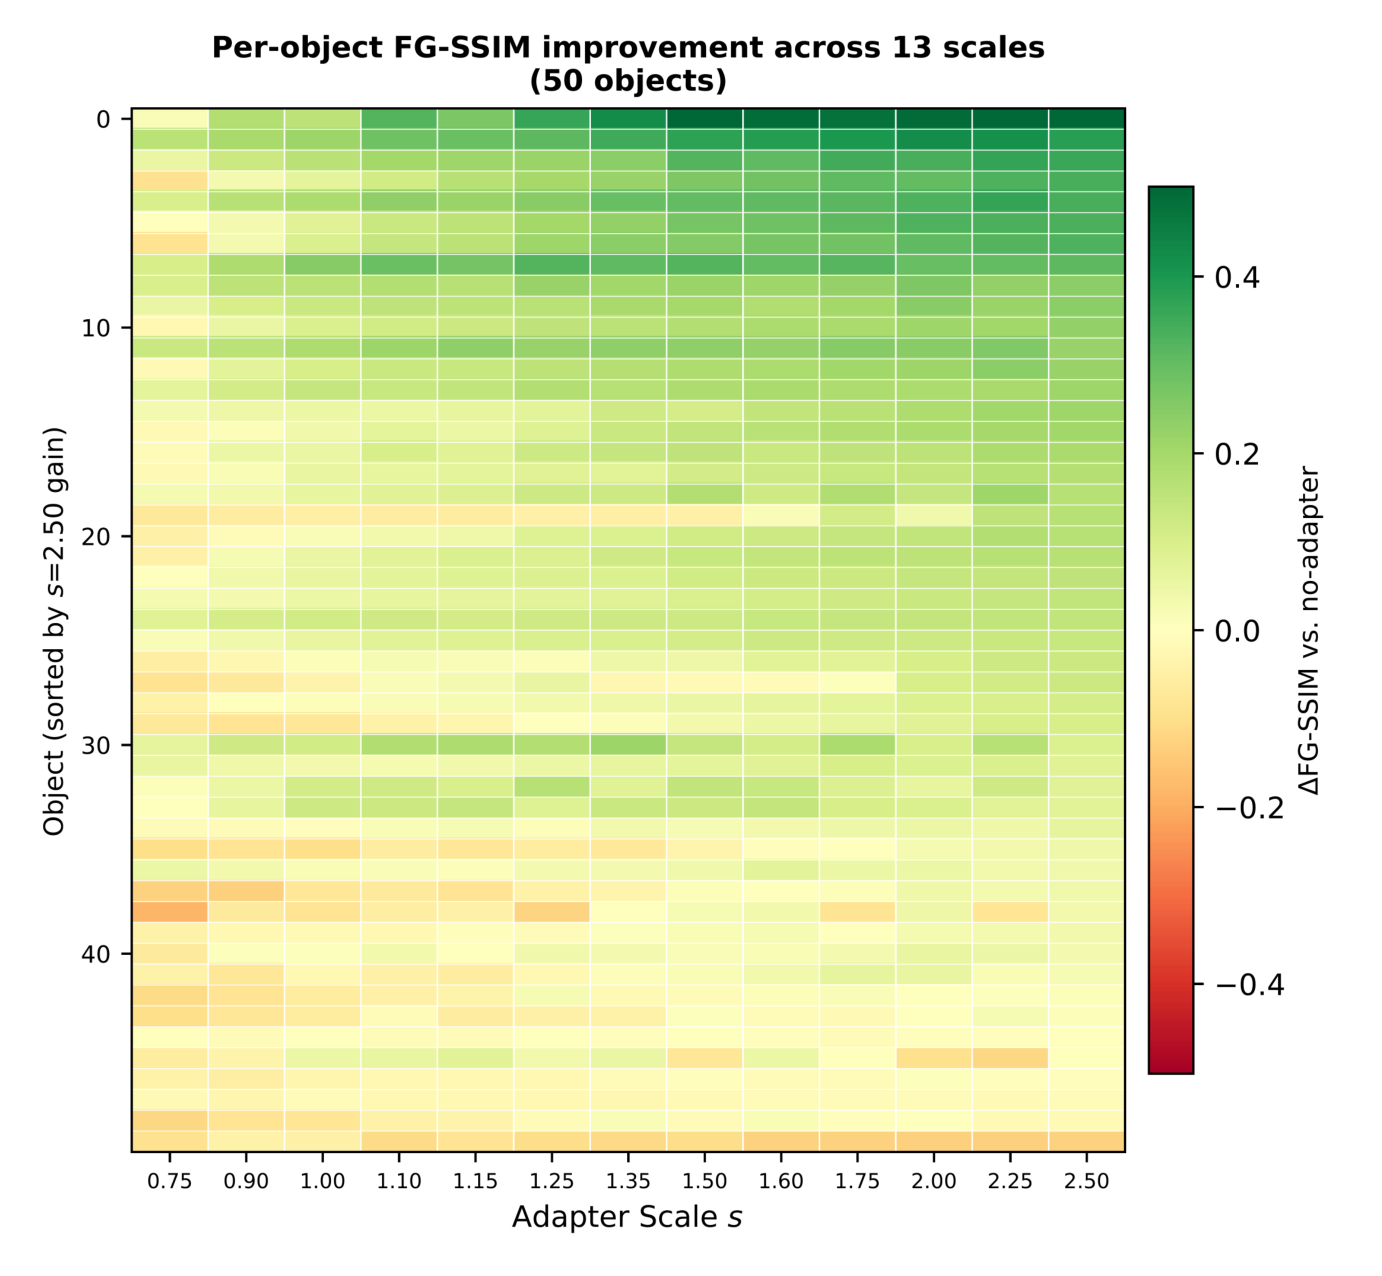
\includegraphics[width=\columnwidth]{fig3.pdf}
\caption{Historical per-object $\Delta$FG-SSIM heatmap reproduced from the 01549 submission (50 objects, 13 scales). The plot illustrates the originally reported response variation; row-level provenance is incomplete, so it is not used for a current population inference.}
\label{fig:heatmap}
\DIFaddendFL \end{figure}

 
 \DIFaddbegin \subsection{C3 Development Record and Current Evaluation}
\DIFaddend \label{subsec:c3}

  \DIFaddbegin \DIFadd{The submitted paper records }\DIFaddend 17   \DIFaddbegin \DIFadd{uniform}\DIFaddend , layer-wise  , and timestep-conditioned  
 \DIFaddbegin \DIFadd{variants on a 24-object development probe and identifies C3 as its chosen profile. This study question remains relevant: does a stage-dependent request offer a useful control setting beyond a single global scale? Because the complete historical row-level data and selection provenance are not available in the current authority, the original Table~\ref{tab:probe} and Figure~\ref{fig:pareto} are retained as historical development records, not as a verified ranking or proof of optimality. Fresh C evaluates the recorded C3 profile without another schedule search}\DIFaddend .

\begin{table}[t]
\centering
  \DIFaddbeginFL \caption{Representative values reported for the historical 24-object, 17-variant development probe. The full candidate set is shown in Figure~\ref{fig:pareto}. The underlying row-level outputs and selection-time provenance are not available for independent reanalysis; the table records the submitted development result and does not establish an optimum.}
\DIFaddendFL \label{tab:probe}
\footnotesize\setlength{\tabcolsep}{3pt}
  \DIFaddbeginFL \begin{tabular}{llcc}
\DIFaddendFL \toprule
Variant &   \DIFaddbeginFL \DIFaddFL{Reported category }\DIFaddendFL & $\Delta$FG-SSIM   & $\Delta$Lap Var   \\
\midrule
C4 & Late-stage high & 0.105 & $-$0.0120   \\
C2 & Timestep   \DIFaddbeginFL \DIFaddFL{schedule }\DIFaddendFL & 0.104 & $-$0.0110   \\
B2 & Layer-wise   \DIFaddbeginFL \DIFaddFL{schedule }\DIFaddendFL & 0.090 & $-$0.0135   \\
A\_s2.00 & Uniform & 0.087 & $-$0.0062   \\
C3   & Mid-stage high & 0.084 & $-$0.0006   \\
A\_s2.25 & Uniform & 0.079 & $-$0.0096   \\
A\_s2.50 & Uniform & 0.078 & $-$0.0108   \\
B6 & Layer-wise   \DIFaddbeginFL \DIFaddFL{schedule }\DIFaddendFL & 0.000 & $-$0.0027   \\
\bottomrule
\end{tabular}
\end{table}

  \DIFaddbegin \DIFadd{The original table and plot use shape and texture-variation proxies to describe the development choice. They do not establish that texture was faithful to the reference, nor that }\DIFaddend C3   \DIFaddbegin \DIFadd{was the unique best candidate. In this revision}\DIFaddend , C3 is   \DIFaddbegin \DIFadd{therefore described as the historical profile carried forward for matched evaluation, not as a theorem-derived or globally optimal schedule}\DIFaddend .

The  
 \DIFaddbegin \DIFadd{recorded profile uses Equation~\ref{eq:tcas} with $(s_e,s_m,s_l)=(1.25,2.50,1.25)$. This is an inference-time instruction on the existing adapter path; no weights are trained. Its tested value is task- and implementation-specific.
}\DIFaddend 

  \DIFaddbeginFL \begin{figure*}[!t]
\DIFaddendFL \centering
  \DIFaddbegin 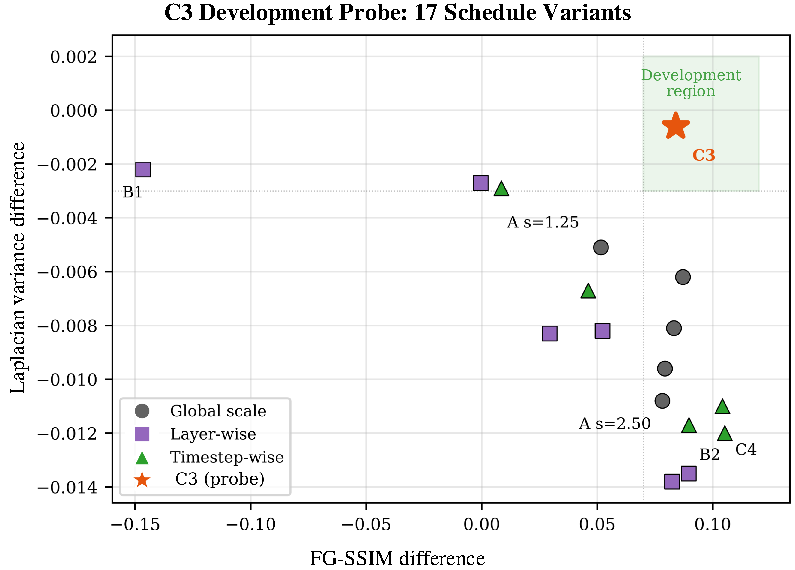
\includegraphics[width=0.78\textwidth]{figures/fig7_c3_development.pdf}
\caption{Historical 17-variant development probe from the submitted 01549 paper (24 objects). The axes show changes in FG-SSIM and Laplacian variance; variance is a texture-variation diagnostic, not a fidelity measure. “C3” identifies the selected historical profile, not an optimum or general schedule law. The green region records the historical selection region, not a validated quality threshold. The candidate-level outputs are unavailable for independent reanalysis.}
\label{fig:pareto}
\end{figure*}
\DIFaddend 

  \DIFaddbegin \DIFadd{The source Figure~5 (26-object texture ratios) is not included as an active result because its object IDs, selection trace, and metric lineage are incomplete. The original 24-object Table~3 is moved to Supplementary Section S10 as a verbatim historical diagnostic, with no texture-fidelity or population inference. Both source assets remain preserved in the authenticated submission and forensic archive; neither decision removes the fixed-scale research question or the development record of }\DIFaddend C3  \DIFaddbegin \DIFadd{.
}

\subsection{Large-Scale Matched Image-Space Evaluation}
\label{subsec:largescale}

\paragraph{Reported main-adapter result in 01549}
\DIFadd{The authenticated 01549 main-table result reports pooled full-image PSNR of 18.86 dB for }\DIFaddend C3   \DIFaddbegin \DIFadd{and 17.90 dB for Fixed High, a historical $+0.96$ dB difference on the original 300-object pool, which includes the 24 development objects. It belongs to the original main-table checkpoint and is not a probe-disjoint estimate. The archived pooled values do not include the object-paired rows needed to reconstruct a paired confidence interval. Fresh C uses a separately frozen retrained checkpoint and paired foreground-masked metrics, so it is a distinct test rather than a numerical reproduction of this historical estimate. The original blinded preference evidence is reported in Section~\ref{subsec:preference}.
}\DIFaddend 

  \DIFaddbegin \DIFadd{Fresh C is a revision-era matched image-space study on $N=300$ objects. Its primary run contains No Adapter, global fixed-low (GFL), global fixed-high (GFH), and the historical C3 profile. A separate addendum evaluates Generic Linear and a layer-conditioned low--low--high temporal profile (LLH) on the same 300 object identifiers; it is not an independent cohort. All conditions within a run share the object, reference/target inputs, six target views, initial latents, and seed. Object is the inferential unit. The frozen evaluator scores each saved 3$\times$2 six-view composite once per object; paired analysis uses these object-level scores.
}\DIFaddend 

  \DIFaddbegin \DIFadd{The registered primary contrast is }\DIFaddend C3   \DIFaddbegin \DIFadd{minus GFL on foreground PSNR (FG-PSNR). The point estimate is $+0.52$~dB (95\% percentile-bootstrap CI $[+0.40,+0.64]$); C3 is higher on 206/300 objects (68.7\%), with median paired difference $+0.554514$~dB. Registered secondary endpoints are reported with the multiplicity treatment and full paired statistics in Supplementary Section S2. PSNR, LPIPS, and SSIM quantify image-space agreement on their respective endpoints; they are not direct measures of texture fidelity or 3D material quality}\DIFaddend .

This   \DIFaddbegin \DIFadd{primary contrast changes more than temporal placement. Across the 50 steps, the applied deep and middle scale sums are 82.5 each for }\DIFaddend C3   \DIFaddbegin \DIFadd{and 62.5 each for GFL; the shallow sum is 40 for both after the native 0.8 cap. The Fresh C estimate therefore supports the recorded C3 intervention relative to GFL under this wrapper, but cannot be attributed to timing alone or interpreted as a pure schedule-shape effect}\DIFaddend .

 
 \DIFaddbeginFL \begin{table*}[t]
\DIFaddendFL \centering
  \DIFaddbeginFL \caption{Fresh C image-space condition means. The primary run contains No Adapter, GFL, GFH, and C3. Generic Linear and LLH are revision-era addendum conditions evaluated on the same object identifiers, not a second independent cohort. Values are means across objects of the frozen evaluator score computed once on each 3$\times$2 six-view composite.}
\label{tab:freshc-absolute}
\scriptsize\setlength{\tabcolsep}{4pt}
\begin{tabular}{lccccc}
\DIFaddendFL \toprule
  \DIFaddbeginFL \DIFaddFL{Method }\DIFaddendFL &   \DIFaddbeginFL \DIFaddFL{$N$ }\DIFaddendFL &   \DIFaddbeginFL \DIFaddFL{FG-PSNR$\uparrow$ }\DIFaddendFL &   \DIFaddbeginFL \DIFaddFL{FG-LPIPS$\downarrow$ }\DIFaddendFL &   \DIFaddbeginFL \DIFaddFL{FG-SSIM$\uparrow$ }& \DIFaddFL{Edge-SSIM$\uparrow$ }\DIFaddendFL \\
\midrule
\DIFaddbeginFL \multicolumn{6}{l}{Primary run} \\
\DIFaddFL{No Adapter }& \DIFaddFL{300 }& \DIFaddFL{6.9779 }& \DIFaddFL{0.2288 }& \DIFaddFL{0.4086 }& \DIFaddFL{0.4314 }\\
\DIFaddFL{GFL }& \DIFaddFL{300 }& \DIFaddFL{11.3077 }& \DIFaddFL{0.2051 }& \DIFaddFL{0.3500 }& \DIFaddFL{0.4728 }\\
\DIFaddFL{GFH }& \DIFaddFL{300 }& \DIFaddFL{12.5777 }& \DIFaddFL{0.1891 }& \DIFaddFL{0.4201 }& \DIFaddFL{0.4961 }\\
\DIFaddendFL C3 \DIFaddbeginFL \DIFaddFL{(TCAS) }\DIFaddendFL &   \DIFaddbeginFL \DIFaddFL{300 }\DIFaddendFL &   \DIFaddbeginFL \DIFaddFL{11.8301 }\DIFaddendFL &   \DIFaddbeginFL \DIFaddFL{0.1998 }\DIFaddendFL &   \DIFaddbeginFL \DIFaddFL{0.3746 }& \DIFaddFL{0.4773 }\DIFaddendFL \\
  \DIFaddbeginFL \midrule
\multicolumn{6}{l}{Same-cohort revision-era addendum} \\
\DIFaddFL{Generic Linear }\DIFaddendFL &   \DIFaddbeginFL \DIFaddFL{300 }\DIFaddendFL &   \DIFaddbeginFL \DIFaddFL{12.4230 }\DIFaddendFL &   \DIFaddbeginFL \DIFaddFL{0.1862 }\DIFaddendFL &   \DIFaddbeginFL \DIFaddFL{0.4026 }& \DIFaddFL{0.4880 }\DIFaddendFL \\
  \DIFaddbeginFL \DIFaddFL{LLH }\DIFaddendFL &   \DIFaddbeginFL \DIFaddFL{300 }\DIFaddendFL &   \DIFaddbeginFL \DIFaddFL{12.4506 }\DIFaddendFL &   \DIFaddbeginFL \DIFaddFL{0.1876 }\DIFaddendFL &   \DIFaddbeginFL \DIFaddFL{0.3911 }& \DIFaddFL{0.4863 }\DIFaddendFL \\
  \DIFaddbeginFL \bottomrule
\end{tabular}
\end{table*}

\begin{table*}[t]
\centering
\caption{Fresh C paired mean differences (A minus B) and pointwise 95\% object-bootstrap CIs. Positive PSNR/SSIM and negative LPIPS favour A. C3--No Adapter/GFH are post hoc; the addendum shares object IDs. Full adjusted families are in Supplement S2.}
\label{tab:freshc-contrasts}
\scriptsize\setlength{\tabcolsep}{3pt}
\begin{tabular}{lcccc}
\toprule
\DIFaddFL{Contrast }& \DIFaddFL{FG-PSNR (dB) }& \DIFaddFL{FG-LPIPS }\DIFaddendFL & \DIFaddbeginFL \DIFaddFL{FG-SSIM }& \DIFaddFL{Edge-SSIM }\\
\midrule
\DIFaddFL{C3 }\DIFaddendFL $-$   \DIFaddbeginFL \DIFaddFL{GFL }& \DIFaddFL{$+0.522\ [0.404,0.641]$ }& \DIFaddFL{$-0.005345\ [-0.006326,-0.004403]$ }& \DIFaddFL{$+0.02453\ [0.02120,0.02805]$ }\DIFaddendFL & \DIFaddbeginFL \DIFaddFL{$+0.004494\ [0.003411,0.005586]$ }\\
\DIFaddFL{C3 }\DIFaddendFL $-$   \DIFaddbeginFL \DIFaddFL{No Adapter }\DIFaddendFL &   \DIFaddbeginFL \DIFaddFL{$+4.852\ [4.553,5.142]$ }\DIFaddendFL &   \DIFaddbeginFL \DIFaddFL{$-0.02905\ [-0.03352,-0.02464]$ }& \DIFaddFL{$-0.03401\ [-0.04214,-0.02591]$ }& \DIFaddFL{$+0.04586\ [0.04114,0.05054]$ }\DIFaddendFL \\
  \DIFaddbeginFL \DIFaddFL{C3 $-$ GFH }& \DIFaddFL{$-0.748\ [-0.890,-0.607]$ }\DIFaddendFL & \DIFaddbeginFL \DIFaddFL{$+0.01070\ [0.008889,0.012554]$ }& \DIFaddFL{$-0.04553\ [-0.04937,-0.04165]$ }& \DIFaddFL{$-0.01881\ [-0.02083,-0.01678]$ }\\
\DIFaddFL{C3 }\DIFaddendFL $-$   \DIFaddbeginFL \DIFaddFL{Generic Linear }\DIFaddendFL & \DIFaddbeginFL \DIFaddFL{$-0.593\ [-0.837,-0.351]$ }& \DIFaddFL{$+0.01351\ [0.01160,0.01549]$ }& \DIFaddFL{$-0.02810\ [-0.03197,-0.02439]$ }& \DIFaddFL{$-0.01069\ [-0.01300,-0.00850]$ }\\
\DIFaddFL{LLH }\DIFaddendFL $-$   \DIFaddbeginFL \DIFaddFL{C3 }\DIFaddendFL &   \DIFaddbeginFL \DIFaddFL{$+0.621\ [0.391,0.855]$ }\DIFaddendFL &   \DIFaddbeginFL \DIFaddFL{$-0.01214\ [-0.01386,-0.01048]$ }& \DIFaddFL{$+0.01658\ [0.01311,0.02003]$ }& \DIFaddFL{$+0.009033\ [0.006867,0.011296]$ }\\
\DIFaddFL{LLH $-$ Generic Linear }& \DIFaddFL{$+0.028\ [-0.015,0.070]$ }& \DIFaddFL{$+0.001372\ [0.000762,0.002081]$ }& \DIFaddFL{$-0.01152\ [-0.01337,-0.00996]$ }& \DIFaddFL{$-0.001660\ [-0.002096,-0.001256]$ }\DIFaddendFL \\
\bottomrule
\end{tabular}
  \DIFaddbegin \end{table*}
\DIFaddend 

  \DIFaddbegin \begin{figure*}[t]
\centering
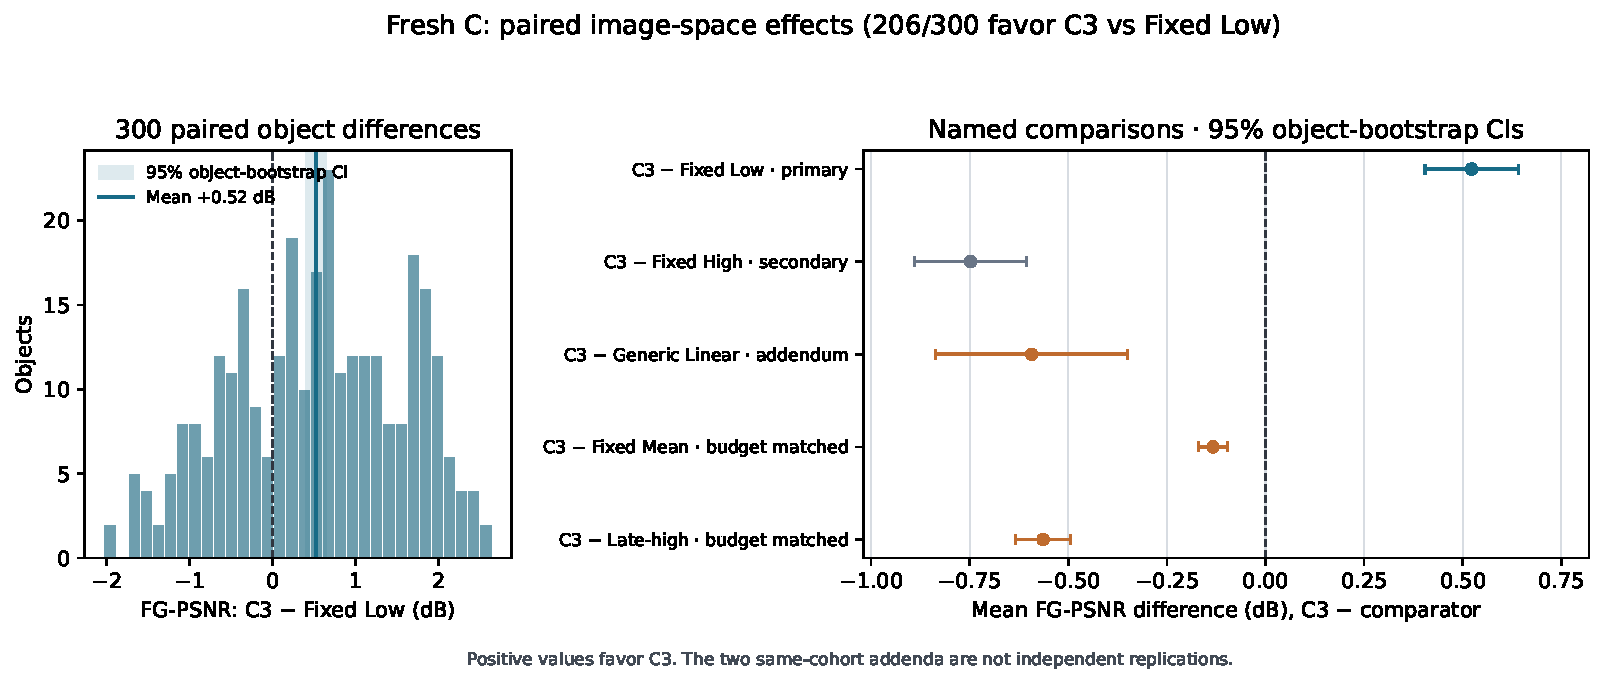
\includegraphics[width=\textwidth]{figures/fig7_freshc_paired_effects.pdf}
\caption{Fresh C paired FG-PSNR differences. The left panel shows all 300 C3--Fixed Low object differences; the right panel shows named mean contrasts and pointwise 95\% object-bootstrap intervals. Positive values favor C3. The Fixed Mean and Late-high comparisons are same-cohort, post-inspection allocation analyses, not independent replications; multiplicity-adjusted results are in Supplementary Section S16.}
\label{fig:freshc-effects}
\end{figure*}

\DIFadd{On this UID-disjoint cohort, the recorded }\DIFaddend C3   \DIFaddbegin \DIFadd{intervention improves mean FG-PSNR relative to Fixed Low under the common Fresh C protocol. The comparison is tied to its stated checkpoint, inputs, seed policy, and native-cap semantics; the complete estimates appear in Tables~\ref{tab:freshc-absolute}--\ref{tab:freshc-contrasts}. Stronger controls produce distinct rankings: Fixed High and Generic Linear have more favorable means than }\DIFaddend C3   \DIFaddbegin \DIFadd{on all four image endpoints, while Fixed Mean and Late-high exceed C3 on FG-PSNR in the equal-budget comparison. The C3--Generic Linear median and object-win count are also reported with the full paired table. These results identify a comparator-specific gain and a measurable endpoint trade-off}\DIFaddend .

  \DIFaddbegin \DIFadd{Fresh C evaluates image-space agreement rather than material fidelity. Figure~\ref{fig:c3compare} gives complete views and shared crops for a fixed-scale comparison and a Generic Linear counterexample; the examples are illustrative, while the cohort tables carry the quantitative result.
}\DIFaddend 

  \DIFaddbegin \begin{figure*}[!t]
\centering
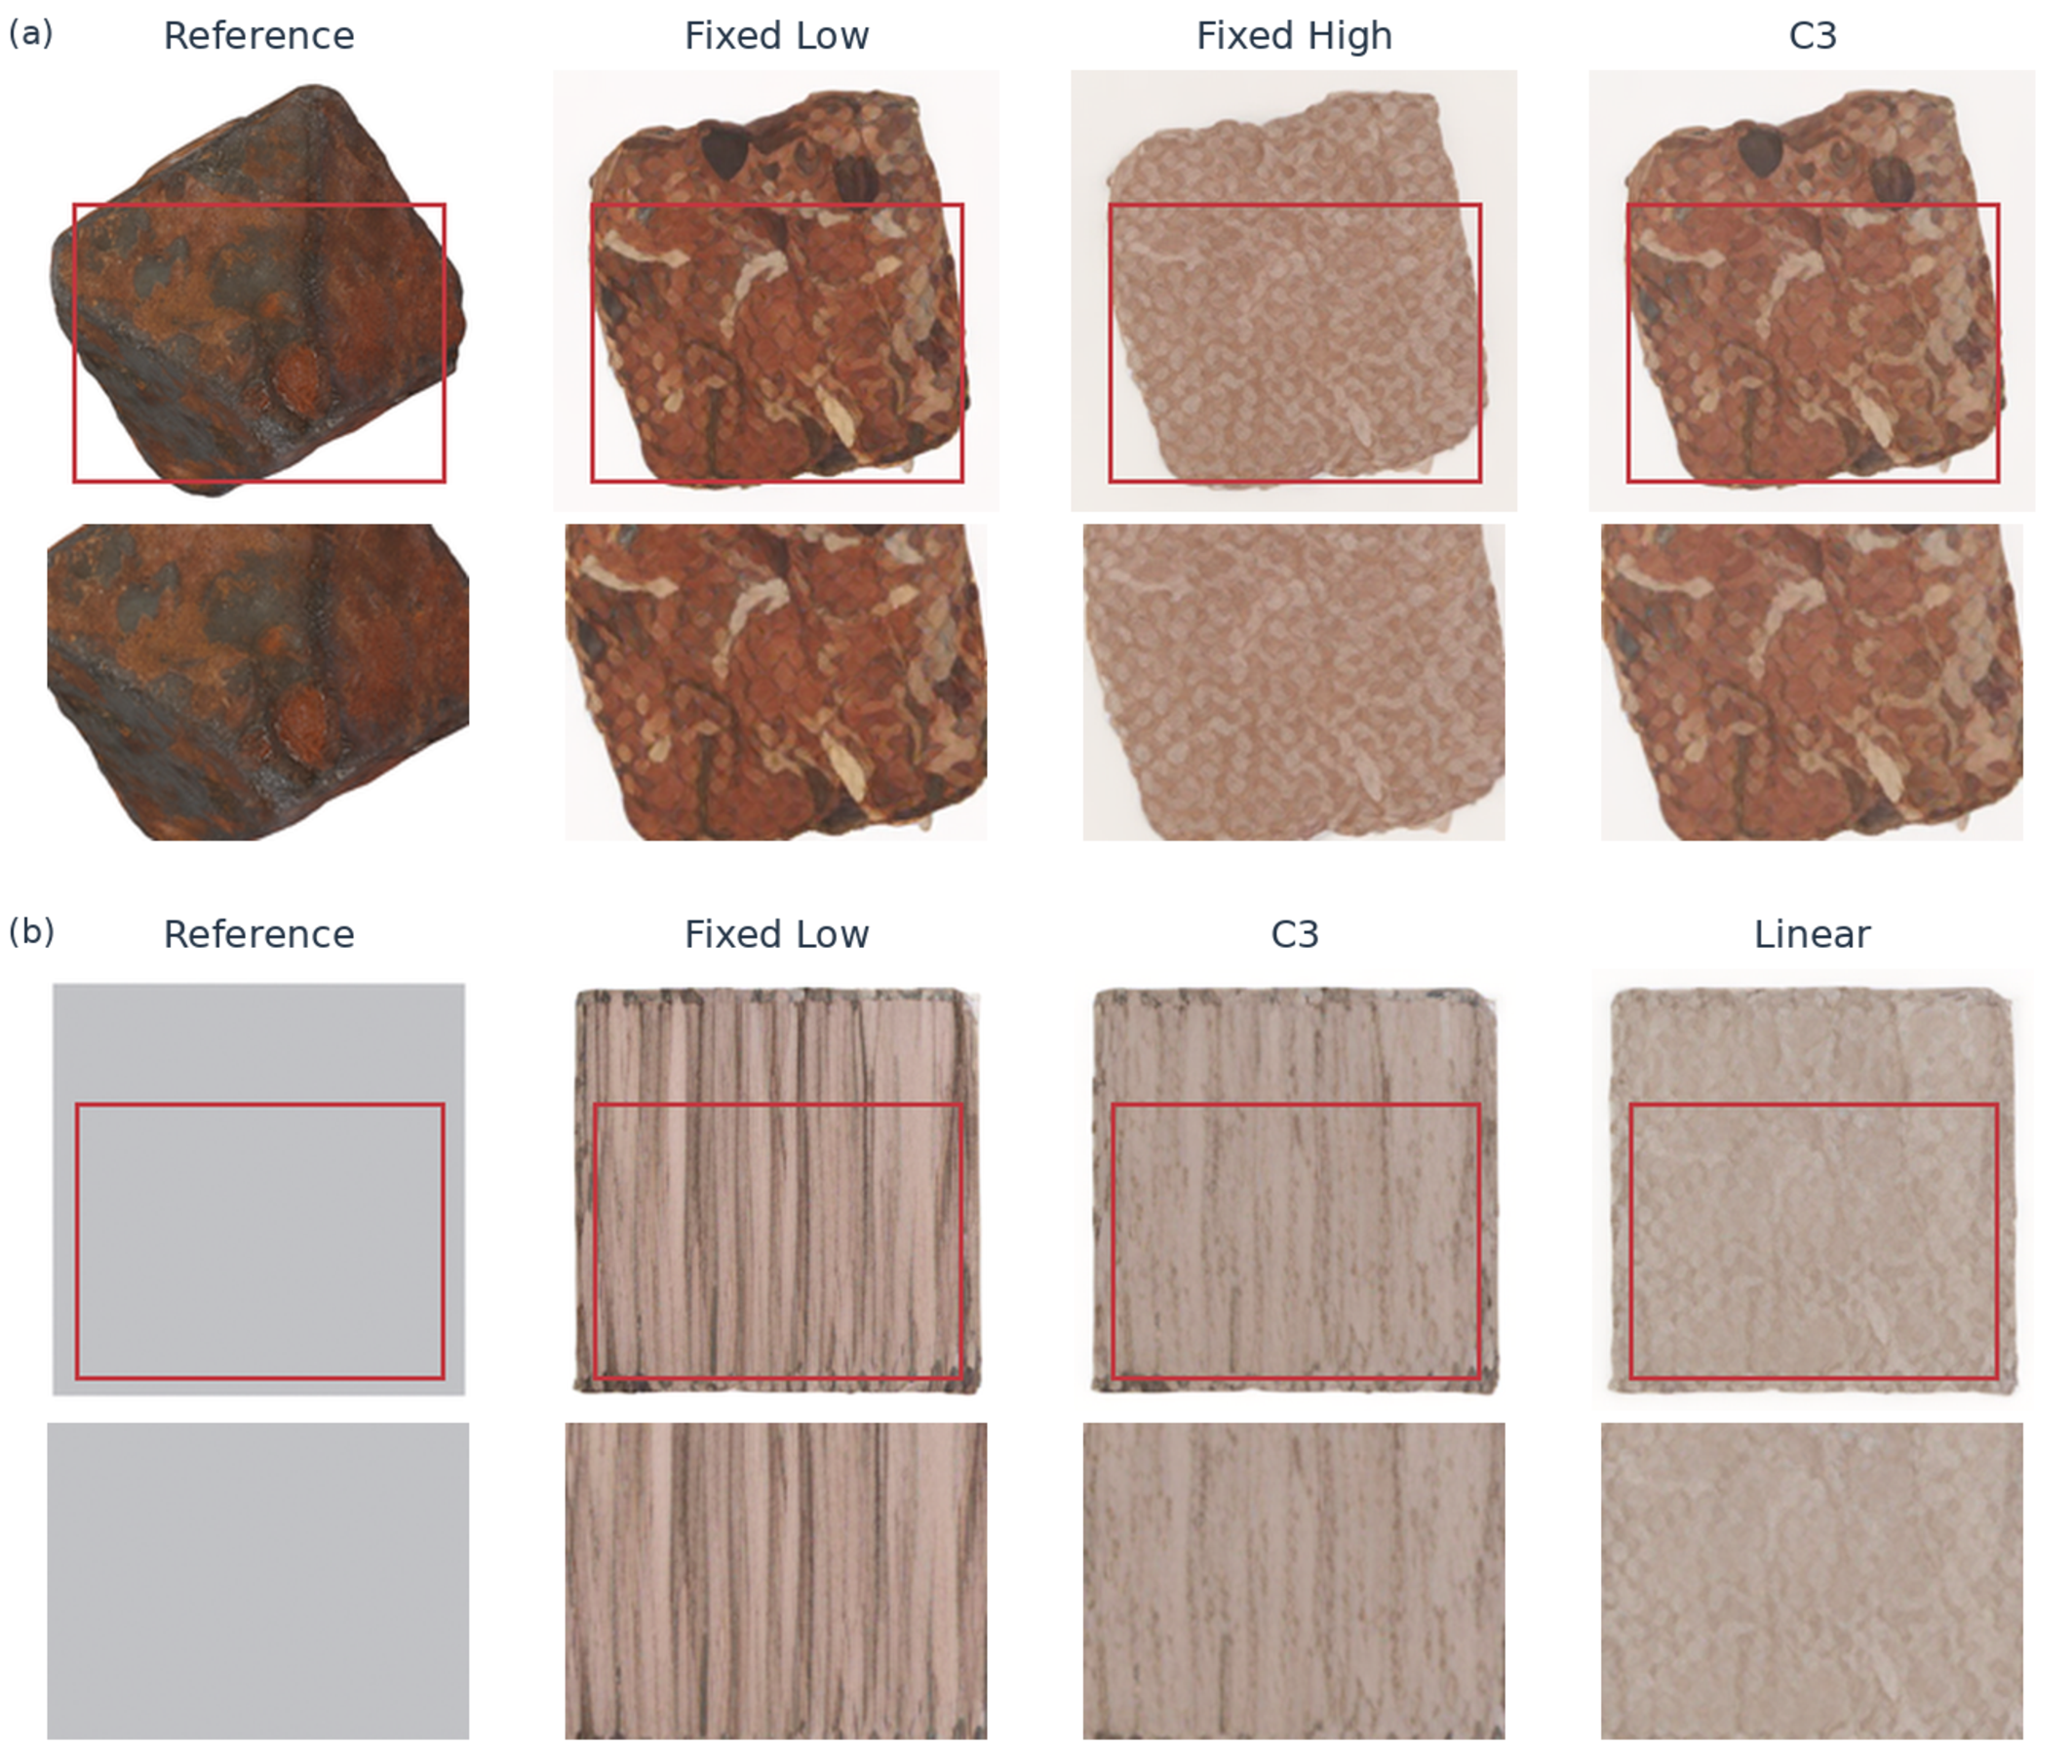
\includegraphics[width=\textwidth]{figures/fig5_freshc_context_roi.pdf}
\caption{Fresh C view 0: (a) Octa\`edre, fixed-scale comparison; (b) Cube 01, Linear counterexample. Columns share the same camera, object, seed and display frame. Red boxes mark the identical pixel crop enlarged below. C3--Linear object-level differences in (b) are $-3.491$ dB FG-PSNR and $+0.08172$ FG-LPIPS. Added patterns differ from the reference despite changes in texture variation. These outcome-selected examples do not estimate prevalence; credits are in Supplementary Table S1.}
\label{fig:c3compare}
\end{figure*}
\DIFaddend 


  \DIFaddbegin \subsection{Applied-Scale Budget and Temporal Placement}
\label{subsec:temporal-placement}

\DIFadd{Fresh C compares the recorded }\DIFaddend C3   \DIFaddbegin \DIFadd{profile with GFL under the same frozen checkpoint, runner, seed policy, inputs, and target views. Its applied deep/middle scale sums are 82.5 for }\DIFaddend C3   \DIFaddbegin \DIFadd{and 62.5 for GFL, while the shallow sum is 40 for both after the 0.8 cap. The registered C3--GFL improvement therefore combines a change in middle-third strength with a larger per-group nominal budget; it does not isolate temporal placement.
}

\DIFadd{A separate post-inspection placement analysis used the clean-v2 strict-276 cohort and a common runner within that run. It is not the Fresh C cohort, and it is not an independent replication of the historical }\DIFaddend 24-object   \DIFaddbegin \DIFadd{selection probe. Temporal L--L--H means low requests during early and middle steps and high requests during late steps; it uses a different shallow-group control from Fresh C's layer-conditioned LLH addendum. The latter requests (1.25,1.25,2.50) in deep/middle and (0.50,0.50,0.75) in shallow; the older global placement comparison keeps shallow capped at 0.8. Neither is identical to the new 16-step Late-high condition. With 50 steps, the strict-276 run assigns 17/16/17 steps to the three windows. C3 and temporal L--L--H have near-matched applied-scale sums (82.50 versus 83.75 in deep and middle; 40 in shallow), but their post-scale residual magnitudes are not matched}\DIFaddend .

  \DIFaddbeginFL \begin{table*}[t]
\DIFaddendFL \centering
  \DIFaddbeginFL \scriptsize
\DIFaddendFL \setlength{\tabcolsep}{4pt}
  \DIFaddbeginFL \caption{Post-inspection strict-276 placement analysis. Entries are C3 minus temporal L--L--H with pointwise 95\% object-bootstrap intervals; positive PSNR/SSIM and negative LPIPS differences favor C3. Temporal L--L--H is favored on all six formal endpoints. The analysis is separate from Fresh C, and its scalar sums do not match realized residual dose.}
\label{tab:temporal-placement}
\begin{tabular}{lcc}
\DIFaddendFL \toprule
  \DIFaddbeginFL \DIFaddFL{Endpoint }\DIFaddendFL &   \DIFaddbeginFL \DIFaddFL{Mean difference }[\DIFaddFL{95\% CI}] \DIFaddendFL &   \DIFaddbeginFL \DIFaddFL{Direction }\DIFaddendFL \\
\midrule
  \DIFaddbeginFL \DIFaddFL{Full-view PSNR (dB) }\DIFaddendFL &   \DIFaddbeginFL \DIFaddFL{$-0.268100$ }[\DIFaddFL{$-0.311101,-0.227797$}] \DIFaddendFL &   \DIFaddbeginFL \DIFaddFL{L--L--H }\\
\DIFaddFL{FG-PSNR (dB) }\DIFaddendFL &   \DIFaddbeginFL \DIFaddFL{$-0.177084$ }[\DIFaddFL{$-0.230539,-0.130784$}] \DIFaddendFL &   \DIFaddbeginFL \DIFaddFL{L--L--H }\DIFaddendFL \\
  \DIFaddbeginFL \DIFaddFL{FG-SSIM }\DIFaddendFL &   \DIFaddbeginFL \DIFaddFL{$-0.008851$ }[\DIFaddFL{$-0.011455,-0.006291$}] \DIFaddendFL &   \DIFaddbeginFL \DIFaddFL{L--L--H }\\
\DIFaddFL{Edge-SSIM }\DIFaddendFL &   \DIFaddbeginFL \DIFaddFL{$-0.035301$ }[\DIFaddFL{$-0.036581,-0.034031$}] \DIFaddendFL &   \DIFaddbeginFL \DIFaddFL{L--L--H }\DIFaddendFL \\
  \DIFaddbeginFL \DIFaddFL{FG-LPIPS }\DIFaddendFL &   \DIFaddbeginFL \DIFaddFL{$+0.001896$ }[\DIFaddFL{$+0.001205,+0.002578$}] \DIFaddendFL &   \DIFaddbeginFL \DIFaddFL{L--L--H }\\
\DIFaddFL{Full-view LPIPS }\DIFaddendFL &   \DIFaddbeginFL \DIFaddFL{$+0.008658$ }[\DIFaddFL{$+0.007465,+0.009831$}] \DIFaddendFL &   \DIFaddbeginFL \DIFaddFL{L--L--H }\DIFaddendFL \\
\bottomrule
\end{tabular}
  \DIFaddbegin \end{table*}
\DIFaddend 

  \DIFaddbegin \DIFadd{Against the fixed-mean profile}\DIFaddend , C3  \DIFaddbegin \DIFadd{'s strict-276 FG-PSNR difference is $+0.502875$~dB (95\% CI $[+0.462018,+0.542244]$)}\DIFaddend . These results show   \DIFaddbegin \DIFadd{sensitivity to the tested stage allocation, not a universally preferred placement or an equal-realized-dose effect}\DIFaddend .

  \DIFaddbegin \DIFadd{Fresh B and Core-7 remain separate retrospective sensitivity analyses in Supplementary Sections S3, S5 }\DIFaddend and   \DIFaddbegin \DIFadd{S21; they are not pooled with Fresh C or used to replicate the historical headline.
}

\subsection{Matched Stage Allocation at Equal Applied Budget}
\label{subsec:matched-budget300}
\DIFadd{The six-condition matrix contains 1,800 object--condition rows, with complete input-hash and common-seed checks. It is a post-inspection addendum on Fresh C's }\DIFaddend 300 objects  \DIFaddbegin \DIFadd{, not an independent holdout. Early-, middle-, and late-high allocate the same 16 high steps to updates 0--15, 17--32, and 34--49. Deep and middle use low 1.25 and high 2.50; shallow remains capped at 0.8. Fixed mean uses 1.65 before the same cap. Thus all four allocation conditions have per-group applied sums (82.5, 82.5, 40), or 205 in total. Fixed Low and Fixed High are separate strength controls and do not share that budget. Generic Linear remains a strong practical baseline in Table~\ref{tab:freshc-absolute}, rather than being silently treated as equal-budget}\DIFaddend .

  \DIFaddbeginFL \begin{table*}[t]
\DIFaddendFL \centering  \DIFaddbeginFL \scriptsize\setlength{\tabcolsep}{4pt}
\caption{Fully matched Fresh C control means ($N=300$ per condition). Timing and fixed-mean rows share exactly the same per-layer applied-scale sums. This same-cohort addendum is post-inspection.}
\label{tab:matched-budget300}
\begin{tabular}{lrrrrr}
\DIFaddendFL \toprule
  \DIFaddbeginFL \DIFaddFL{Control }\DIFaddendFL &   \DIFaddbeginFL \DIFaddFL{FG-PSNR}\DIFaddendFL $\uparrow$ &   \DIFaddbeginFL \DIFaddFL{FG-LPIPS$\downarrow$ }& \DIFaddFL{FG-SSIM}\DIFaddendFL $\uparrow$ &   \DIFaddbeginFL \DIFaddFL{Edge-SSIM}\DIFaddendFL $\uparrow$ \DIFaddbeginFL & \DIFaddFL{PSNR winners }\DIFaddendFL \\
\midrule
  \DIFaddbeginFL \DIFaddFL{GFH / Fixed High }\DIFaddendFL &   \DIFaddbeginFL \DIFaddFL{12.58 }\DIFaddendFL &   \DIFaddbeginFL \DIFaddFL{0.1891 }\DIFaddendFL &   \DIFaddbeginFL \DIFaddFL{0.4201 }\DIFaddendFL &   \DIFaddbeginFL \DIFaddFL{0.4961 }\DIFaddendFL &   \DIFaddbeginFL \DIFaddFL{172 }\DIFaddendFL \\
  \DIFaddbeginFL \DIFaddFL{GFL / Fixed Low }\DIFaddendFL &   \DIFaddbeginFL \DIFaddFL{11.31 }\DIFaddendFL &   \DIFaddbeginFL \DIFaddFL{0.2051 }\DIFaddendFL &   \DIFaddbeginFL \DIFaddFL{0.3500 }& \DIFaddFL{0.4728 }& \DIFaddFL{37 }\DIFaddendFL \\
 

 \DIFaddbeginFL \DIFaddFL{Fixed Mean }\DIFaddendFL &   \DIFaddbeginFL \DIFaddFL{11.96 }\DIFaddendFL &   \DIFaddbeginFL \DIFaddFL{0.1978 }\DIFaddendFL &   \DIFaddbeginFL \DIFaddFL{0.3864 }& \DIFaddFL{0.4843 }& \DIFaddFL{2 }\DIFaddendFL \\
  \DIFaddbeginFL \DIFaddFL{Early-high }\DIFaddendFL &   \DIFaddbeginFL \DIFaddFL{11.33 }\DIFaddendFL &   \DIFaddbeginFL \DIFaddFL{0.2045 }\DIFaddendFL &   \DIFaddbeginFL \DIFaddFL{0.3696 }& \DIFaddFL{0.4765 }& \DIFaddFL{25 }\DIFaddendFL \\
  \DIFaddbeginFL \DIFaddFL{C3 / Middle-high }\DIFaddendFL &   \DIFaddbeginFL \DIFaddFL{11.83 }\DIFaddendFL &   \DIFaddbeginFL \DIFaddFL{0.1998 }\DIFaddendFL &   \DIFaddbeginFL \DIFaddFL{0.3746 }& \DIFaddFL{0.4773 }& \DIFaddFL{0 }\DIFaddendFL \\
  \DIFaddbeginFL \DIFaddFL{Late-high }\DIFaddendFL &   \DIFaddbeginFL \DIFaddFL{12.39 }\DIFaddendFL &   \DIFaddbeginFL \DIFaddFL{0.1951 }\DIFaddendFL &   \DIFaddbeginFL \DIFaddFL{0.3788 }& \DIFaddFL{0.4914 }& \DIFaddFL{64 }\DIFaddendFL \\
\bottomrule
\end{tabular}
  \DIFaddbegin \end{table*}
\DIFaddend 

  C3  
 \DIFaddbegin \DIFadd{minus Fixed Mean is $-0.13$ dB (pointwise 95\% object-bootstrap CI $[-0.17,-0.10]$). }\DIFaddend C3   \DIFaddbegin \DIFadd{minus Late-high is $-0.56$ dB (pointwise 95\% object-bootstrap CI $[-0.63,-0.49]$). C3 minus Early-high is $+0.50$ dB (pointwise }\DIFaddend 95  \DIFaddbegin \DIFadd{\% object-bootstrap CI $[+0.37,+0.62]$). }\DIFaddend C3   \DIFaddbegin \DIFadd{also trails Fixed Mean and Late-high on FG-LPIPS, FG-SSIM and Edge-SSIM. Complete paired endpoint distributions, 50,000 object-bootstrap resamples and post hoc Holm-adjusted contrasts are supplied in Supplementary Section S16. The original stage-centered contrast, C3 minus the mean of Early-high and Late-high FG-PSNR, is $-0.034$ dB (95\% CI $[-0.117,+0.051]$; paired sign-flip $p=0.4324$). It likewise does not support a middle-window advantage; the later pairwise analysis is explicitly post-inspection. The rank count is specific to FG-PSNR and these six conditions; it does }\DIFaddend not establish a   \DIFaddbegin \DIFadd{universal quality winner. We retain }\DIFaddend C3  \DIFaddbegin \DIFadd{'s development identity but reject a generally optimal middle window. Residual amplitudes differ along the resulting trajectories: this restricts a further mechanism claim, while the equal-budget allocation comparison still measures the total effect of stage allocation}\DIFaddend .

  \DIFaddbegin \subsection{Layer-by-Window Sensitivity}
\label{subsec:layerwindow}
\DIFaddend 

  \DIFaddbegin \DIFadd{The A2 and A3b maps test response heterogeneity over three adapter groups and five denoising windows. Their object-cluster statistics describe variation within the tested interventions; they are not effect estimates for a dose-independent schedule mechanism}\DIFaddend .

\begin{table}[t]
\centering
  \DIFaddbeginFL \scriptsize
\setlength{\tabcolsep}{3pt}
\caption{Object-cluster tests of the observed layer-by-window response maps. A2 is exploratory; A3b is retrospective Fresh B sensitivity because the preserved history cannot authenticate pre-run availability of its lock. Interaction share and cell RMSE summarize the observed map, not a causal effect.}
\label{tab:layerwindow-main}
\begin{tabular}{llrrr}
\DIFaddendFL \toprule
  \DIFaddbeginFL \DIFaddFL{Map, cohort }\DIFaddendFL &   \DIFaddbeginFL \DIFaddFL{Endpoint }\DIFaddendFL &   \DIFaddbeginFL \DIFaddFL{Wald $W(8)$ }\DIFaddendFL &   \DIFaddbeginFL \DIFaddFL{Reported $p$ }& \DIFaddFL{Share; cell RMSE }\DIFaddendFL \\
\midrule
  \DIFaddbeginFL \DIFaddFL{A2, $N=300$ }\DIFaddendFL &   \DIFaddbeginFL \DIFaddFL{FG-PSNR }\DIFaddendFL &   \DIFaddbeginFL \DIFaddFL{1879.963 }\DIFaddendFL &   \DIFaddbeginFL \DIFaddFL{$<10^{-300}$ }& \DIFaddFL{56.8\%; 0.1222~dB }\DIFaddendFL \\
  \DIFaddbeginFL \DIFaddFL{A2, $N=300$ }\DIFaddendFL &   \DIFaddbeginFL \DIFaddFL{FG-LPIPS }\DIFaddendFL &   \DIFaddbeginFL \DIFaddFL{481.081 }\DIFaddendFL &   \DIFaddbeginFL \DIFaddFL{$8.04\times10^{-99}$ }& \DIFaddFL{43.5\%; 0.001695 }\DIFaddendFL \\
  \DIFaddbeginFL \DIFaddFL{A3b, $N=150$ }\DIFaddendFL &   \DIFaddbeginFL \DIFaddFL{FG-PSNR }\DIFaddendFL &   \DIFaddbeginFL \DIFaddFL{525.700 }\DIFaddendFL &   \DIFaddbeginFL \DIFaddFL{$3.43\times10^{-107}$ }& \DIFaddFL{36.0\%; 0.0205~dB }\\
\DIFaddFL{A3b, $N=150$ }& \DIFaddFL{FG-LPIPS }& \DIFaddFL{225.015 }& \DIFaddFL{$5.37\times10^{-43}$ }& \DIFaddFL{14.0\%; 0.000342 }\DIFaddendFL \\
\bottomrule
\end{tabular}
\end{table}

  \DIFaddbegin \DIFadd{The response maps describe heterogeneity under the tested controls. Cross-layer raw norms and retrospective complexity associations do not establish an optimal schedule or a causal mechanism; full diagnostics are in Supplementary Sections S3--S4, S12 and S21.
}

\subsection{Appearance and Color Failure Analysis}
\label{subsec:appearance-color}

\DIFadd{The selected color diagnosis contains 26 failure-enriched objects: six earlier figure cases and 20 Fresh C panels. It is not a random sample, a new holdout, or a population estimate. No Adapter, GFL, and LLH were compared on the same inputs, checkpoint, and runner with six target views per object (78 object-condition records}\DIFaddend ). The   \DIFaddbegin \DIFadd{following paired object-bootstrap intervals are descriptive (20,000 resamples; seed 61008}\DIFaddend ), and   \DIFaddbegin \DIFadd{no confirmatory multiplicity family was defined.
}

\begin{figure*}[t]
\centering
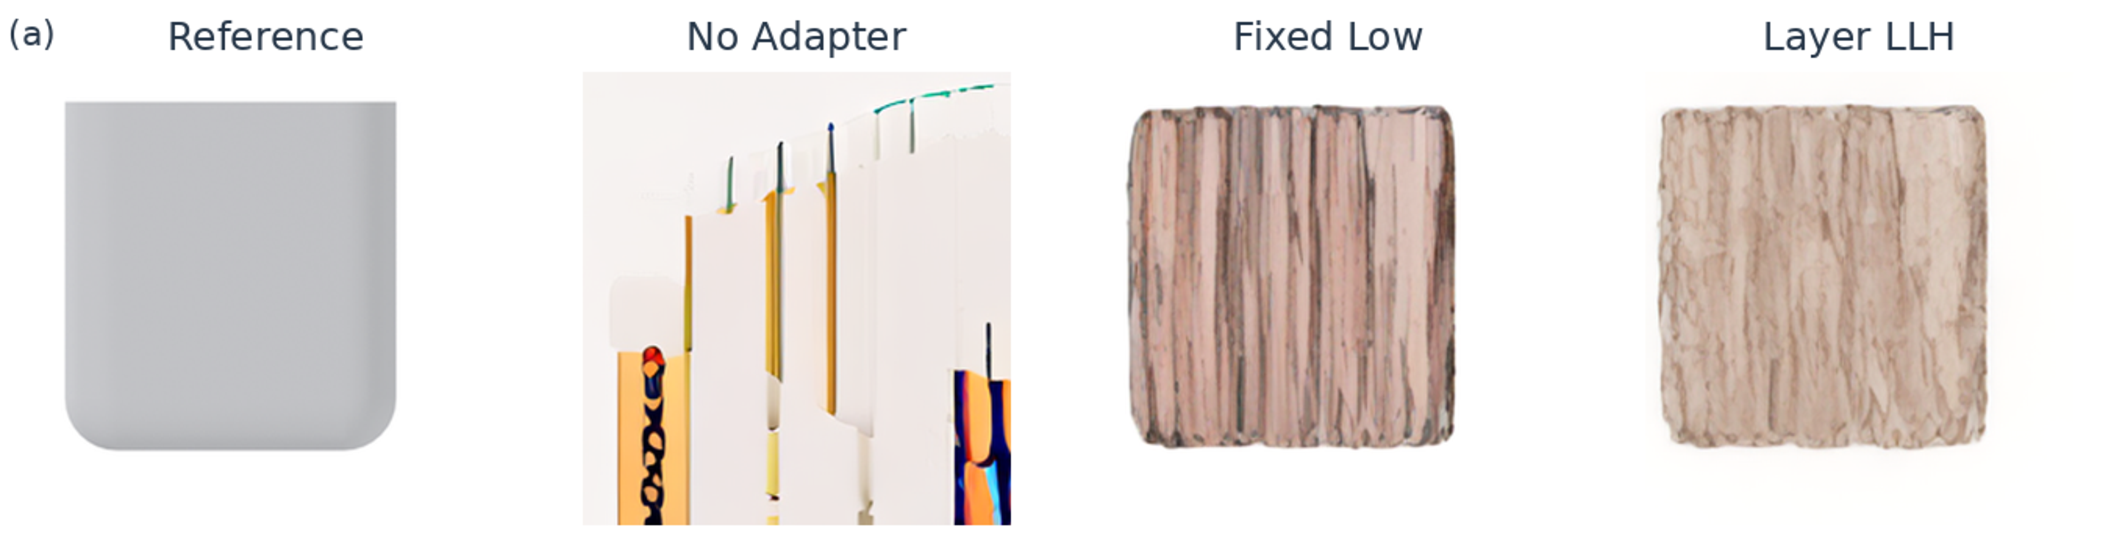
\includegraphics[width=\textwidth]{figures/fig6_color_diagnostic_freshc_context_roi.pdf}
\caption{Fresh C view 0, E5-5-2. The same frame shows reference, disabled adapter, Fixed Low and layer LLH. Geometry conditioning changes alignment and patterned appearance, but the brown texture does not reproduce the gray reference. This previously viewed example was selected by an existing LPIPS stratum, not for color. It is not a reconstruction of the legacy purple-shift panels; attribution is in Supplementary Table S1.}
\label{fig:color-failure}
\end{figure*}

\begin{table}[t]
\centering
\scriptsize
\setlength{\tabcolsep}{3pt}
\caption{Selected paired results from the failure-enriched 26-object color diagnosis. Negative CIEDE2000 differences indicate lower reference-color error for the first condition. The set is descriptive and does not estimate population prevalence.}
\label{tab:color-summary}
\begin{tabular}{p{2.3cm}p{3.3cm}p{1.3cm}}
\toprule
\DIFaddFL{Contrast }& \DIFaddFL{Mean CIEDE2000 difference }[\DIFaddFL{95\% CI}] & \DIFaddFL{Objects }\\
\midrule
\DIFaddFL{GFL -- No Adapter }& \DIFaddFL{$-19.654$ }[\DIFaddFL{$-26.370,-13.248$}] & \DIFaddFL{24/26 lower }\\
\DIFaddFL{LLH -- GFL }& \DIFaddFL{$+3.583$ }[\DIFaddFL{$+0.462,+6.712$}] & \DIFaddFL{-- }\\
\bottomrule
\end{tabular}
\end{table}

\DIFadd{In the selected 26-object diagnosis, GFL reduces mean reference-color error relative to No Adapter by 19.65 CIEDE2000 units (}\DIFaddend 95\%   \DIFaddbegin \DIFadd{paired interval $[-26.37,-13.25]$; 24/26 favorable). LLH increases color error relative to GFL by 3.58 while reducing local variation. These paired results distinguish conditioning response from reference fidelity; the set is failure-enriched and does not estimate prevalence. Figure~\ref{fig:color-failure} shows a traced Fresh C example, not a reconstruction of the two unmapped legacy purple-shift panels. No repair is claimed.
}

\DIFadd{Historical bake cohorts, execution-stack checks and unsuccessful repair candidates are documented in Supplementary Sections S13, S18--S19 and S21. They are supporting diagnostics rather than additional evidence for }\DIFaddend C3   \DIFaddbegin \DIFadd{quality. The new calibrated bake pilot is evaluated separately below}\DIFaddend .

  \DIFaddbegin \paragraph{Fresh C full-object and same-ROI examples.}
\label{subsec:visual}

\DIFadd{The 26-object texture audit is not used as cohort-level evidence because its object-level source records and executable metric definition are unavailable. The historical variation proxies are retained only as diagnostics in Supplementary Section S12.
}

\DIFadd{Figure~\ref{fig:qualitative} shows two rights-cleared Fresh C cases selected from five previously illustrated objects: each favors C3 over Fixed Low on the three object-level composite metrics and on displayed view 0. Shared local crops are enlarged below each complete object view. These outcome-selected cases illustrate the measured direction; Table~\ref{tab:freshc-absolute} and Figure~\ref{fig:freshc-effects} report the cohort evidence. Figure~\ref{fig:c3compare} provides a fixed-scale comparison and a Generic Linear counterexample; Supplementary Figure~S1 retains the six-view Boat comparison.
}

\begin{figure*}[!t]
\centering
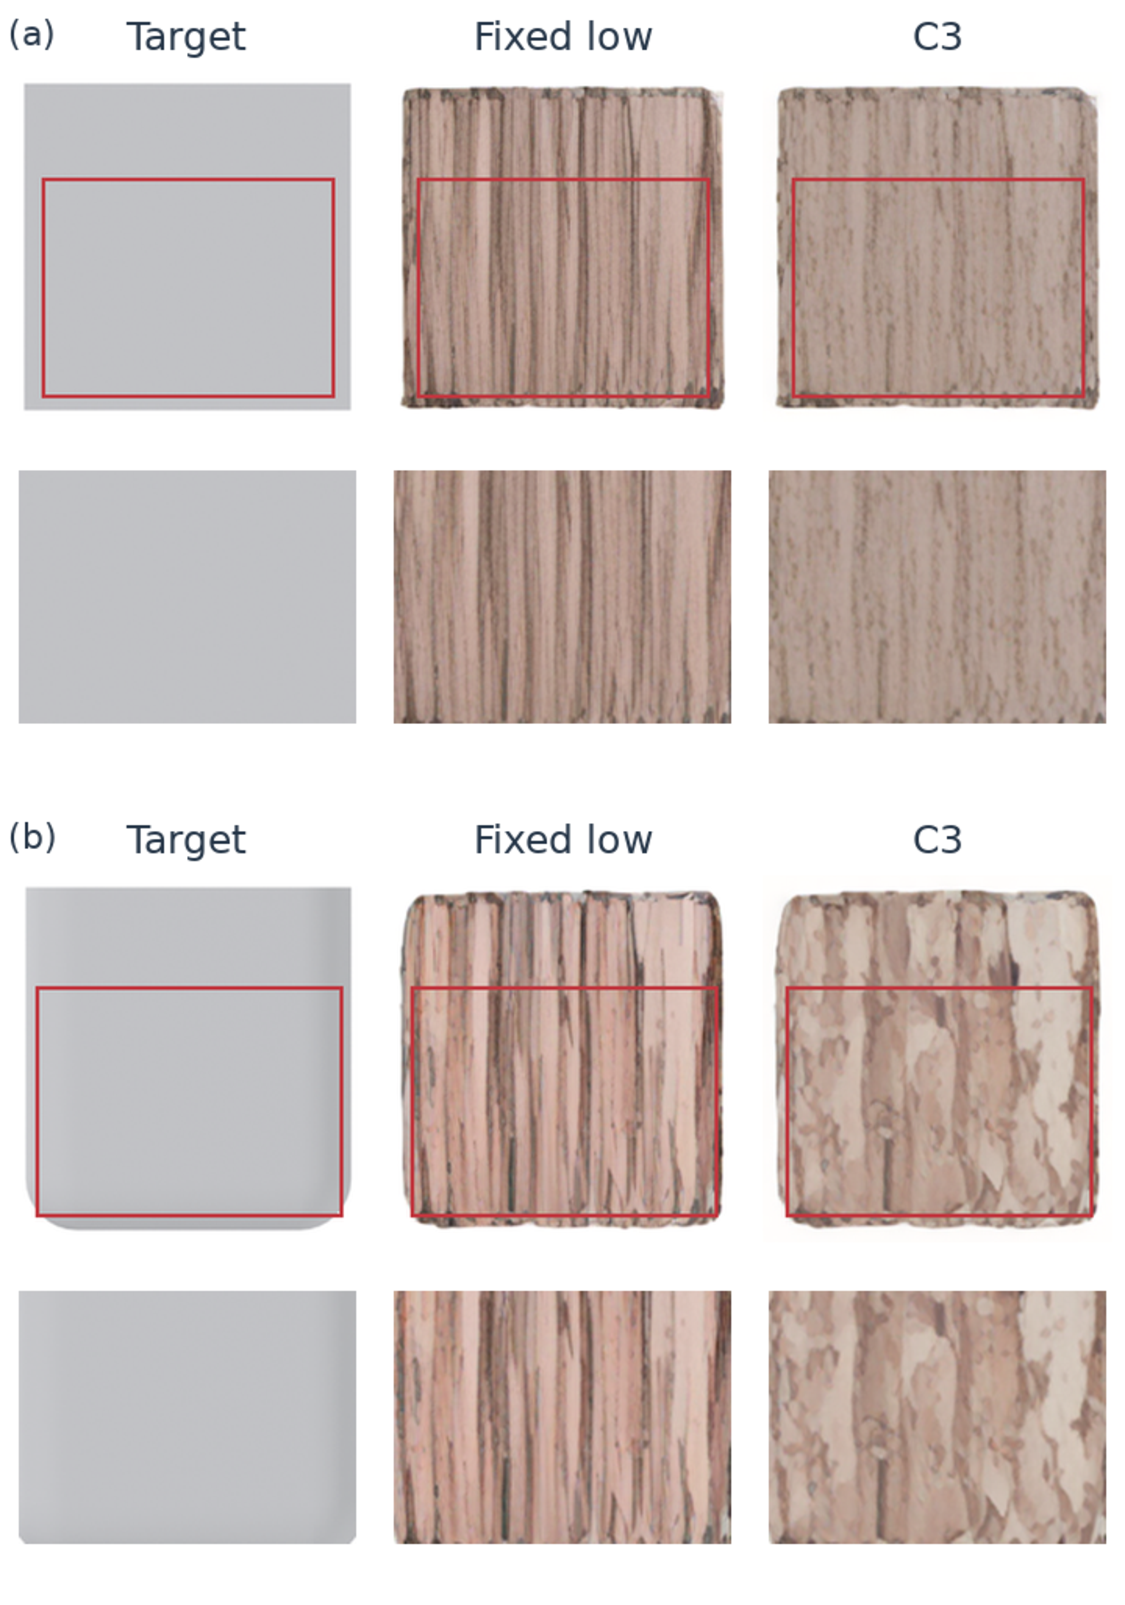
\includegraphics[width=0.78\textwidth]{figures/fig7_metric_favorable.pdf}
\caption{Metric-selected Fresh C examples: (a) Cube 01 and (b) E5-5-2. C3--Fixed Low object-level differences on the full 3$\times$2 composite are FG-PSNR $+1.79$ and $+1.26$ dB, FG-LPIPS $-0.0243$ and $-0.0327$, and FG-SSIM $+0.185$ and $+0.162$, respectively. Each strip shows the target render, complete view 0 and a shared pixel crop enlarged below. The target renders are low-variation; these examples illustrate the image-space metric contrast, not texture fidelity. Object-level values are computed on all six views together, and displayed-view scoring is a selection diagnostic. Both examples favor C3 on the three composite metrics and on view 0; they illustrate the measured direction, not its prevalence. Full-cohort results are in Table~\ref{tab:freshc-absolute} and Figure~\ref{fig:freshc-effects}. Credits are in Supplementary Table S1.}
\label{fig:qualitative}
\end{figure*}




\subsection{First-round cluster-aware preference study}
\label{subsec:preference}

\DIFadd{The 01549 first-round revision reported }\DIFaddend a blinded three-alternative forced-choice   study on 30 objects   \DIFaddbegin \DIFadd{with 24 participants. Participants compared conservative fixed-scale, aggressive fixed-scale, and C3 outputs for }\DIFaddend texture naturalness, shape consistency,   \DIFaddbegin \DIFadd{and overall quality; condition order was randomized per trial. Each criterion had }\DIFaddend 720   first-choice decisions  \DIFaddbegin \DIFadd{. Table~\ref{tab:preference} reports the aggregate counts; participant-level responses are not redistributed with this revision}\DIFaddend .

  \DIFaddbeginFL \begin{table}[t]
\DIFaddendFL \centering  \DIFaddbeginFL \scriptsize
\caption{First-round 01549 3AFC results retained as reported. Percentages use 720 decisions per criterion; preference is not a measure of reference texture fidelity.}
\DIFaddendFL \label{tab:preference}
  \DIFaddbeginFL \setlength{\tabcolsep}{3pt}
\DIFaddendFL \begin{tabular}{lccc}
\toprule
Method & Texture naturalness   & Shape consistency   & Overall quality   \\
\midrule
  \DIFaddbeginFL \DIFaddFL{$s=1.25$ }\DIFaddendFL &   \DIFaddbeginFL \DIFaddFL{332/720 (46.1\%) }\DIFaddendFL & 96/720 (13.3\%) & 176/720 (24.4\%) \\
  \DIFaddbeginFL \DIFaddFL{$s=2.50$ }\DIFaddendFL & 104/720 (14.4\%) &   \DIFaddbeginFL \DIFaddFL{331/720 (46.0\%) }\DIFaddendFL & 126/720 (17.5\%) \\
C3 (TCAS) & 284/720 (39.4\%) & 293/720 (40.7\%) &   \DIFaddbeginFL \DIFaddFL{418/720 (58.1\%) }\DIFaddendFL \\
\bottomrule
\end{tabular}
\end{table}
  

The  
 \DIFaddbegin \DIFadd{reported analysis used }\DIFaddend a two-level   \DIFaddbegin \DIFadd{participant/object bootstrap with }\DIFaddend 10  \DIFaddbegin \DIFadd{,}\DIFaddend 000 resamples  . C3's overall-quality share   \DIFaddbegin \DIFadd{was }\DIFaddend 58.1\% (95\% CI   \DIFaddbegin [\DIFadd{50.1\%, 65.8\%}]\DIFadd{); its differences from }\DIFaddend the conservative and aggressive baselines   \DIFaddbegin \DIFadd{were +33.6 points (CI }[\DIFadd{19.3, 47.2}]\DIFadd{) and +40.6 }\DIFaddend points (CI   \DIFaddbegin [\DIFadd{29.4, 51.8}]\DIFadd{). The }\DIFaddend single-criterion advantages   \DIFaddbegin \DIFadd{for texture naturalness and shape consistency had intervals crossing zero. This bounded preference result does not validate texture fidelity, unseen-view quality, or the Fresh C cohort}\DIFaddend .

  \DIFaddbegin \subsection{Calibrated Baked Appearance on New Objects}
\label{subsec:new-bake}
\DIFadd{We froze ten previously unbaked Fresh C objects in UID order using input availability, native UV/material compatibility, triangle-count and camera-mask alignment criteria. Of the 300 screened inputs, only ten passed all criteria before the cutoff; the planned maximum was twenty. The ten are not new to the GeoTex image domain, but their baked outcomes had not been inspected during selection. This is a compatibility-selected pilot, not a representative twenty-object confirmation. Five earlier bake objects are reported separately.
}\DIFaddend 

  \DIFaddbegin \DIFadd{Seven conditions share each object's source mesh, reference, seed, six projection cameras, masks, 256-pixel source resolution, atlas resolution, hole filling and eleven unseen evaluation cameras. Original geometry, UVs and legal base-color material semantics are retained and checked. Unseen cameras do not enter the bake. GT-256 uses the same source resolution, masks and bake parameters and has exactly the same raw atlas coverage as every generated condition. Native REPEAT sampling passes boundary and integer-period tests; pole-view RGB orientation is corrected without rotating raw-camera masks. These calibrations control projection artifacts; evaluation is unlit base color, not PBR fidelity. Supplementary Section~S18 records the checks and object-level data. The Constant 1.0 control is capped at the shallow group and is not the unset-scale GeoTex default. No generated output for that unmodified path is available in this comparison, so the corresponding reviewer request remains partially unresolved.
}\DIFaddend 

  \DIFaddbegin \begin{table}[ht]
\centering\scriptsize
\caption{New ten-object unlit unseen-view bake pilot. Eleven views are averaged per object. Higher PSNR/SSIM and lower LPIPS/CIEDE2000 are favorable. Constant 1.0 is an explicitly capped request, not the unset-scale pipeline. The GT row is a projection calibration control; all seven generated conditions and all ten eligible objects are retained.}
\label{tab:new-bake}
\begin{tabular}{lrrrr}
\toprule \DIFaddFL{Condition }& \DIFaddendFL FG-PSNR  

 \DIFaddbeginFL & \DIFaddFL{FG-LPIPS }& \DIFaddFL{FG-SSIM }& \DIFaddFL{CIEDE2000 }\\
\midrule
\DIFaddFL{GT-256 bake (calibration) }& \DIFaddFL{22.38 }& \DIFaddFL{0.0590 }& \DIFaddFL{0.7683 }& \DIFaddFL{4.44 }\\
\DIFaddFL{Constant 1.0 (capped) }& \DIFaddFL{11.93 }& \DIFaddFL{0.1354 }& \DIFaddFL{0.3504 }& \DIFaddFL{24.18 }\\
\DIFaddFL{Fixed Low }& \DIFaddFL{12.48 }& \DIFaddFL{0.1317 }& \DIFaddFL{0.3835 }& \DIFaddFL{22.71 }\\
\DIFaddFL{Fixed High }& \DIFaddFL{12.29 }& \DIFaddFL{0.1305 }& \DIFaddFL{0.4587 }& \DIFaddFL{23.27 }\\
\DIFaddFL{Fixed Mean }& \DIFaddFL{12.62 }& \DIFaddFL{0.1303 }& \DIFaddFL{0.4193 }& \DIFaddFL{22.32 }\\
\DIFaddendFL C3  

 \DIFaddbeginFL \DIFaddFL{/ Middle-high }& \DIFaddFL{12.48 }& \DIFaddFL{0.1302 }& \DIFaddFL{0.4059 }& \DIFaddFL{22.16 }\\
\DIFaddFL{Late-high }& \DIFaddFL{12.92 }& \DIFaddFL{0.1277 }& \DIFaddFL{0.4259 }& \DIFaddFL{21.65 }\\
\DIFaddFL{Generic Linear }& \DIFaddFL{11.60 }& \DIFaddFL{0.1276 }& \DIFaddFL{0.4458 }& \DIFaddFL{24.71 }\\
\bottomrule\end{tabular}
\end{table}
\DIFaddend 

The  
 \DIFaddbegin \DIFadd{frozen primary contrast was Late-high minus Fixed Mean on unseen-view FG-LPIPS, proposed from the earlier pilot and tested on the ten selected bake objects. Its mean is $-0.00265$ }\DIFaddend ( 

 \DIFaddbegin \DIFadd{95\% object-bootstrap CI $[-0.00414,-0.00137]$; exact paired sign-flip $p=0.00195$), with all ten objects favoring Late-high. Generic Linear has a slightly lower mean LPIPS and lower PSNR, so the bake metrics retain an endpoint trade-off}\DIFaddend .

 
 \DIFaddbegin \DIFadd{C3--Fixed High has mean PSNR $+0.19$}\DIFaddend ~dB (95\% CI   \DIFaddbegin \DIFadd{$[-0.65,+0.87]$) and LPIPS $-0.00036$ ($[-0.00396,+0.00336]$); neither separates under the four-comparison secondary Holm family (both adjusted $p=1$). The SSIM difference favors Fixed High by 0.05274 (95\% CI $[0.03170,0.07459]$; Holm $p=0.00781$). The full pilot results are reported separately from the earlier five-object bake.
}

\DIFadd{Across the seven conditions, generated-view and baked unseen-view rankings are positively associated (mean within-object Spearman $\rho=0.746$--$0.907$); the winning condition changes for LPIPS on 7}\DIFaddend /  \DIFaddbegin \DIFadd{10 objects. Figure~\ref{fig:baked-context} shows the source, GT-256 projection control, and generated bakes. The generated results retain visible color and pattern differences from the source, so this pilot supports relative metric comparisons rather than reference-faithful material recovery.
}

\begin{figure*}[t]
\centering
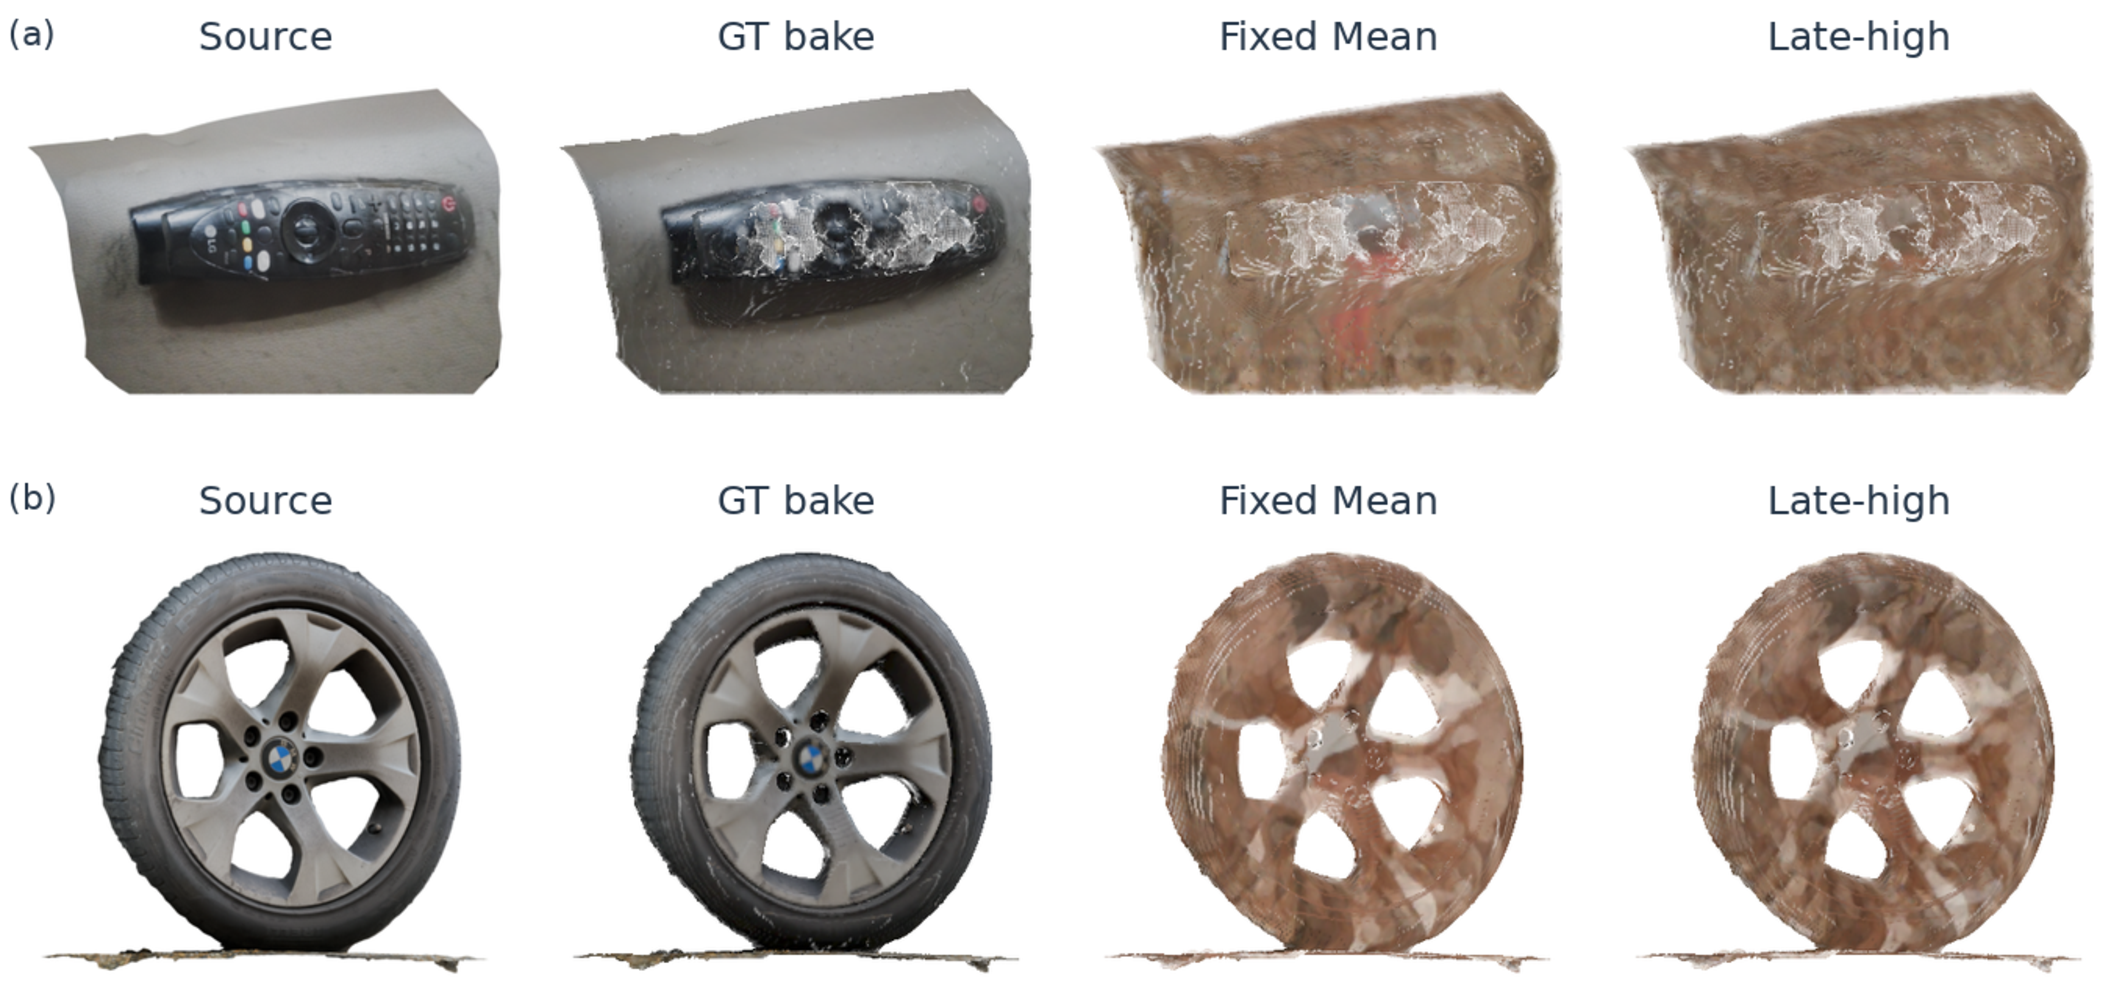
\includegraphics[width=\textwidth]{figures/fig8_baked_unseen_context.pdf}
\caption{Unseen camera 004: (a) LG Remote, (b) Tire. Source and GT-256 bake calibrate projection; Fixed Mean and Late-high isolate the principal comparison. All columns share one display frame, without color/detail editing. GT retains much of the source appearance; generated results retain brown-pattern errors despite a small cohort-level LPIPS improvement. Complete seven-condition comparisons are in Supplementary Figures S2--S8. Credits: mohd.akmal.mahyudin and Koto3D Stephane Vogley, CC Attribution (Supplement S18).}
\label{fig:baked-context}
\end{figure*}

\subsection{Second-Interface Evaluation with Native MV-Adapter}
\label{subsec:new-mva}

\DIFadd{Earlier exploratory MV-Adapter layer}\DIFaddend /  \DIFaddbegin \DIFadd{window panels and the MVDiffusion compatibility panel remain documented in Supplementary Sections S12 and S17. The main second-interface result below is the input-frozen native-camera MV-Adapter comparison; it is reported within that system's own scale definition and albedo target.
}

\DIFadd{The native MV-Adapter matrix contains 50 input-selected objects and seven shared conditions. Outputs were not inspected during input selection; the complete matrix retains all 350 object--condition records, including 13 texture-absent sources with white-albedo targets. The remaining 37 textured objects are a descriptive subset, not a replacement cohort. Native-camera calibration, source-UV checks, and the three-object implementation-identity audit are detailed in Supplementary Section S17; the earlier seven-object archive is kept separate because it used a different camera calibration.
}

\DIFadd{The seven conditions share object inputs, seed, geometry and evaluation code. With 50 steps, low}\DIFaddend /  \DIFaddbegin \DIFadd{high are 0.75}\DIFaddend /  \DIFaddbegin \DIFadd{1.0; each stage-high schedule has 16 high steps, Fixed Mean is 0.83, and Generic Linear is 0.75--0.91. These five mean-matched controls each sum to 41.5 per scaled feature within this interface. Targets are unlit native-camera albedo and are not numerically interchangeable with Fresh C's rendered targets}\DIFaddend .

  \DIFaddbeginFL \begin{table}[ht]
\DIFaddendFL \centering
  \DIFaddbeginFL \scriptsize
\caption{Native-camera MV-Adapter comparison on fifty input-selected objects. Values are per-condition object means; seven controls share inputs, seed, geometry and evaluation. Scales and endpoints are specific to this interface.}
\label{tab:new-mva}
\begin{tabular}{lrrrr}
\DIFaddendFL \toprule
  \DIFaddbeginFL \DIFaddFL{Condition }\DIFaddendFL &   \DIFaddbeginFL \DIFaddFL{FG-PSNR }\DIFaddendFL &   \DIFaddbeginFL \DIFaddFL{FG-LPIPS }\DIFaddendFL &   \DIFaddbeginFL \DIFaddFL{FG-SSIM }\DIFaddendFL &   \DIFaddbeginFL \DIFaddFL{Edge-SSIM }\DIFaddendFL \\
\midrule
  \DIFaddbeginFL \DIFaddFL{Native / Fixed High }\DIFaddendFL &   \DIFaddbeginFL \DIFaddFL{12.60 }\DIFaddendFL &   \DIFaddbeginFL \DIFaddFL{0.1280 }\DIFaddendFL &   \DIFaddbeginFL \DIFaddFL{0.5041 }\DIFaddendFL &   \DIFaddbeginFL \DIFaddFL{0.3526 }\DIFaddendFL \\
  \DIFaddbeginFL \DIFaddFL{Fixed Low }\DIFaddendFL &   \DIFaddbeginFL \DIFaddFL{12.73 }\DIFaddendFL &   \DIFaddbeginFL \DIFaddFL{0.1270 }\DIFaddendFL &   \DIFaddbeginFL \DIFaddFL{0.5066 }\DIFaddendFL &   \DIFaddbeginFL \DIFaddFL{0.3475 }\DIFaddendFL \\
  \DIFaddbeginFL \DIFaddFL{Fixed Mean }\DIFaddendFL &   \DIFaddbeginFL \DIFaddFL{12.68 }\DIFaddendFL &   \DIFaddbeginFL \DIFaddFL{0.1279 }\DIFaddendFL &   \DIFaddbeginFL \DIFaddFL{0.5068 }\DIFaddendFL &   \DIFaddbeginFL \DIFaddFL{0.3509 }\DIFaddendFL \\
  \DIFaddbeginFL \DIFaddFL{Early-high }\DIFaddendFL &   \DIFaddbeginFL \DIFaddFL{12.60 }\DIFaddendFL &   \DIFaddbeginFL \DIFaddFL{0.1296 }\DIFaddendFL &   \DIFaddbeginFL \DIFaddFL{0.5041 }\DIFaddendFL &   \DIFaddbeginFL \DIFaddFL{0.3503 }\DIFaddendFL \\
  \DIFaddbeginFL \DIFaddFL{Middle-high }\DIFaddendFL &   \DIFaddbeginFL \DIFaddFL{12.71 }\DIFaddendFL &   \DIFaddbeginFL \DIFaddFL{0.1262 }\DIFaddendFL &   \DIFaddbeginFL \DIFaddFL{0.5061 }\DIFaddendFL &   \DIFaddbeginFL \DIFaddFL{0.3470 }\\
\DIFaddFL{Late-high }& \DIFaddFL{12.74 }& \DIFaddFL{0.1260 }& \DIFaddFL{0.5075 }& \DIFaddFL{0.3514 }\\
\DIFaddFL{Generic Linear }& \DIFaddFL{12.72 }& \DIFaddFL{0.1263 }& \DIFaddFL{0.5072 }& \DIFaddFL{0.3501 }\DIFaddendFL \\
\bottomrule
\end{tabular}
\end{table}

 
 \DIFaddbegin \DIFadd{The internally frozen primary, Middle-high minus Fixed Mean FG-PSNR, is $+0.029$ dB (95\% object-bootstrap CI $[-0.019,+0.081]$; paired Monte Carlo sign-flip $p=0.281$; 29/50 favorable). The complete matrix therefore supplies a valid native-interface test, while its primary interval does not separate from zero. The remaining 104 pair--metric tests use one Holm family; full contrasts, the textured subset and protocol are in Supplementary Section S17}\DIFaddend .  
 \DIFaddbegin \DIFadd{Endpoint-specific differences, including lower Middle-high Edge-SSIM than Fixed Mean, are retained there}\DIFaddend .

  \DIFaddbegin \begin{figure*}[t]
\centering
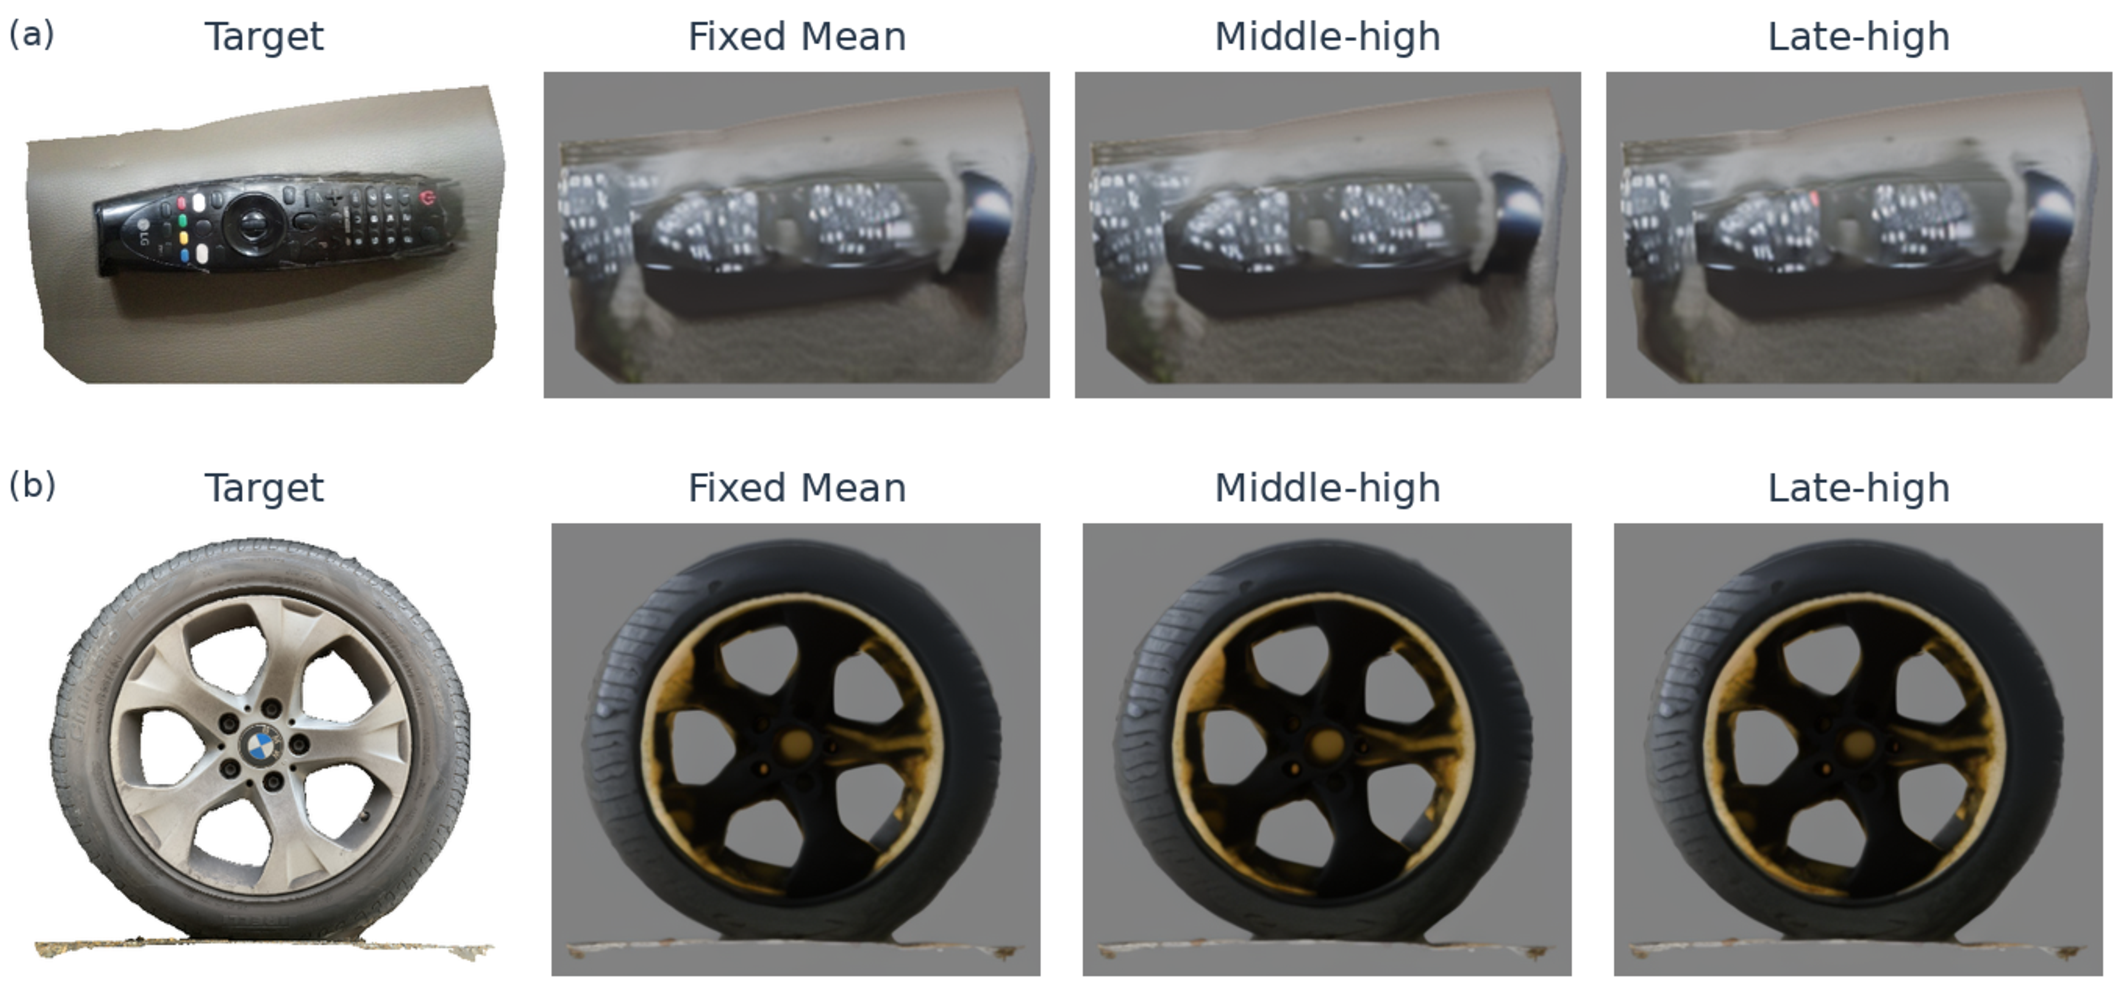
\includegraphics[width=\textwidth]{figures/fig9_mvadapter_native.pdf}
\caption{Native MV-Adapter view 0: (a) LG Remote and (b) Tire. Target, Fixed Mean, Middle-high and Late-high share the native camera and object seed, with the original background and a common crop across conditions. These rights-cleared cases illustrate the output; the full seven-condition matrix and the primary paired estimate are reported in Table~\ref{tab:new-mva} and Supplementary Figure S9. Attribution is in Supplementary Section S18.}
\label{fig:native-mva-visual}
\end{figure*}

\subsection{FAC controlled re-examination reported in 01549}
\label{subsec:facreported}

\DIFadd{A previously reported FAC re-examination found that all seven trained configurations had lower FG-PSNR than TCAS by 1.10--2.94 dB, with at most 48/300 wins; the separate 12-object untrained control had $\Delta$FG-PSNR $=-0.18$ dB (95\% CI }[\DIFadd{$-0.42,+0.05$}]\DIFaddend ).   \DIFaddbegin \DIFadd{These are first-round reported results, not a new training run. The recovered archive lacks a run-bound manifest and weights for a full FAC replay (Supplementary Section S11).
}

\section{Discussion}
\DIFadd{TCAS makes temporal adapter strength an explicit inference-time control on the existing GeoTex residual path. The original blinded study favors }\DIFaddend C3   \DIFaddbegin \DIFadd{for its own stimuli, and Fresh C finds a paired FG-PSNR gain over Fixed Low. Stronger fixed/linear and equal-budget comparisons show that this gain is comparator-specific and that allocation changes endpoint rankings.
}\DIFaddend 

  \DIFaddbegin \DIFadd{The two metric-selected examples in Figure~\ref{fig:qualitative} are consistent with their full-composite and displayed-view metric directions; the full 300-object distribution supports the cohort-level estimate. The calibrated bake pilot adds an unseen-view comparison favoring Late-high over Fixed Mean on FG-LPIPS, while the native MV-Adapter study supplies a distinct second-interface estimate. Together, these experiments characterize inference-time control across preference, image-space, bake, and native-interface evaluations.
}

\DIFadd{A separate post-submission study of per-view guidance projection is documented in Supplementary Section~S22. It evaluates a distinct intervention and is not used as evidence for TCAS or its schedule.
}

\section{Limitations}
\label{sec:limitations}
\DIFadd{Historical 01549, Fresh C, MV-Adapter, and bake results retain separate checkpoints and cohorts. Fresh C is not a numerical reproduction of the historical pooled result; its equal-budget addendum is a same-cohort analysis. The preference study concerns its original stimuli. The bake pilot covers ten technically compatible objects and unlit base color; an unset-scale GeoTex output, validated seam metric, and PBR/relighting study are not included. The native MV-Adapter primary interval includes zero. FAC replay remains limited by missing run-bound training records and weights. Full provenance and scope are in Supplementary Sections S8, S11, S17--S21}\DIFaddend .

\section{Conclusion}
\label{sec:conclusion}
 
 \DIFaddbegin \DIFadd{TCAS provides a training-free temporal control for geometry-adapter strength }\DIFaddend in multi-view   texture generation. The   \DIFaddbegin \DIFadd{original preference study and held-out Fresh C comparison support measured C3 benefits for their tested stimuli and comparator, while the matched-budget controls identify how fixed and late-heavy allocation perform on the same cohort. Calibrated baking and native MV-Adapter testing extend this evaluation to a downstream appearance domain and a distinct conditioning interface. Together, these results provide a concrete, reproducible characterization of temporal adapter control in the tested texturing pipeline}\DIFaddend .

  \DIFaddbegin \section*{\DIFadd{Data availability}}
\DIFaddend 

  \DIFaddbegin \DIFadd{Object-level revision metrics, frozen protocols/configuration records, verified inference and analysis scripts, and the LaTeX source required to rebuild the manuscript and Supplement are included in the author-review package. The standalone reproduction archive supports statistic recomputation without model weights; fresh inference additionally requires the recorded weights, runtime and licensed source assets. The separate projection follow-up in Supplementary Section~S22 is supplied with its frozen cohort, score rows, comparison summaries, and analysis source. Raw generated-image archives, trained checkpoints, source 3D assets whose redistribution rights are not established, and participant-level responses are not included. Additional analysis records may be requested from the corresponding author, subject to licensing, privacy, }\DIFaddend and  

\section*{}
 \DIFaddbegin \DIFadd{archive constraints.
}\DIFaddend 

  \DIFaddbegin \section*{\DIFadd{Declaration of generative AI and AI-assisted technologies in manuscript preparation}}
\DIFadd{OpenAI Codex assisted with revision drafting, implementation and reproducible statistical and figure code. Figure~\ref{fig:overview} is a code-generated vector schematic; the earlier generated conceptual artwork is excluded from this revision. Actual input/output thumbnails and experimental displays come from the recorded research runs and were not retouched with an image-generation tool. Numerical tables are computed from delivered object-level records. Final scientific review, accuracy and responsibility remain with the authors}\DIFaddend .

\section*{Declaration of competing interests}

The authors declare that they have no known competing financial interests or personal relationships that could have appeared to influence the work reported in this paper.


\DIFaddbegin \begingroup
\linespread{0.94}\selectfont
\DIFaddend \begin{thebibliography}{45}
\linespread{0.90}\selectfont\setlength{\itemsep}{-0.6pt}
\bibitem{liu2023zero1to3}
Liu R, Wu R, Van Hoorick B, et al. Zero-1-to-3: Zero-shot one image to 3D object. \textit{Proceedings of the IEEE/CVF International Conference on Computer Vision}, 2023.

\bibitem{shi2023zero123pp}
Shi R, Chen H, Zhang Z, et al. Zero123++: A single image to consistent multi-view diffusion base model. arXiv:2310.15110, 2023.

\bibitem{liu2023syncdreamer}
Liu Y, Lin C, Zeng Z, et al. SyncDreamer: Generating multiview-consistent images from a single-view image. \textit{International Conference on Learning Representations}, 2024.

\bibitem{long2023wonder3d}
Long X, Guo Y C, Lin C, et al. Wonder3D: Single image to 3D using cross-domain diffusion. \textit{Proceedings of the IEEE/CVF Conference on Computer Vision and Pattern Recognition}, 2024.

\bibitem{shi2024mvdream}
Shi Y, Wang P, Ye J, et al. MVDream: Multi-view diffusion for 3D generation. \textit{International Conference on Learning Representations}, 2024.

\bibitem{wang2023imagedream}
Wang P, et al. ImageDream: Image-prompt multi-view diffusion for 3D generation. arXiv:2312.02201, 2023.

\bibitem{xu2024instantmesh}
Xu J, et al. InstantMesh: Efficient 3D mesh generation from a single image with sparse-view large reconstruction models. \textit{Advances in Neural Information Processing Systems}, 2024.

\bibitem{ke2024era3d}
Li P, Liu Y, Long X, et al. Era3D: High-resolution multiview diffusion using efficient row-wise attention. \textit{Advances in Neural Information Processing Systems}, 2024.

\bibitem{chen2023text2tex}
Chen D Z, et al. Text2Tex: Text-driven texture synthesis via diffusion models. \textit{Proceedings of the IEEE/CVF International Conference on Computer Vision}, 2023.

\bibitem{richardson2023texture}
Richardson E, Metzer G, Alaluf Y, et al. TEXTure: Text-guided texturing of 3D shapes. \textit{ACM SIGGRAPH 2023 Conference Proceedings}, 2023.

\bibitem{poole2023dreamfusion}
Poole B, Jain A, Barron J T, Mildenhall B. DreamFusion: Text-to-3D using 2D diffusion. \textit{International Conference on Learning Representations}, 2023.

\bibitem{chen2023fantasia3d}
Chen R, Chen Y, Jiao N, Jia K. Fantasia3D: Disentangling geometry and appearance for high-quality text-to-3D content creation. \textit{Proceedings of the IEEE/CVF International Conference on Computer Vision}, 2023.

\bibitem{shao2025mvpainter}
Shao M, Xiong F, Sun Z, Xu M. MVPainter: Accurate and detailed 3D texture generation via multi-view diffusion with geometric control. arXiv:2505.12635, 2025.

\bibitem{kynkanniemi2024limited}
Kynk\"a\"anniemi T, Aittala M, Karras T, et al. Applying guidance in a limited interval improves sample and distribution quality in diffusion models. \textit{Advances in Neural Information Processing Systems}, 2024.

\bibitem{perla2026survey}
Perla S R K, Zhang H, Mahdavi-Amiri A. Advances in neural 3D mesh texturing: A survey. \textit{Computer Graphics Forum}, 2026, e70392.

\bibitem{guzman2026adaptive}
Guzm\'an J E, Mould D, Paquette E. Adaptive multiresolution exemplar-based texture synthesis on animated fluids. \textit{Computers \& Graphics}, 2026, 134: 104490.

\bibitem{lv2025interpretable}
Lv X, Wu Z, Xu J, et al. Interpretable procedural material graph generation via diffusion models from reference images. \textit{The Visual Computer}, 2025, 41(13): 11195--11205.

\bibitem{zeng2024paint3d}
Zeng X, Chen X, Qi Z, et al. Paint3D: Paint anything 3D with lighting-immersive texture generation. \textit{Proceedings of the IEEE/CVF Conference on Computer Vision and Pattern Recognition}, 2024.

\bibitem{cheng2024mvpaint}
Cheng W, Mu J, Zeng X, et al. MVPaint: Synchronized multi-view diffusion for painting anything 3D. \textit{Proceedings of the IEEE/CVF Conference on Computer Vision and Pattern Recognition}, 2025.

\bibitem{lai2025hunyuan3d}
Zhao Z, Lai Z, Lin Q, et al. Hunyuan3D 2.0: Scaling diffusion models for high resolution textured 3D assets generation. arXiv:2501.12202, 2025.

\bibitem{huang2024mvadapter}
Huang Z, et al. MV-Adapter: Multi-view consistent image generation made easy. \textit{Proceedings of the IEEE/CVF International Conference on Computer Vision}, 2025.

\DIFaddbegin \bibitem{tang2023mvdiffusion}
\DIFadd{Tang S, Zhang F, Chen J, Wang P, Furukawa Y. MVDiffusion: Enabling holistic multi-view image generation with correspondence-aware diffusion. \textit{Advances in Neural Information Processing Systems}, 2023.
}

\DIFaddend \bibitem{liu2024synchronized}
Liu Y X, Xie M S, Liu H Y, Wong T T. Text-guided texturing by synchronized multi-view diffusion. \textit{SIGGRAPH Asia 2024 Conference Papers}, 2024.

\bibitem{xu2026wondertex}
Xu Q, Han X G, Zhang L. WonderTex: Consistent-and-seamless texture generation with text-guided multi-view image diffusion models. \textit{IEEE Transactions on Visualization and Computer Graphics}, 2026, 32(7): 5815--5825.

\bibitem{mou2023t2iadapter}
Mou C, Wang X, Xie L, et al. T2I-Adapter: Learning adapters to dig out more controllable ability for text-to-image diffusion models. \textit{Proceedings of the AAAI Conference on Artificial Intelligence}, 2024.

\bibitem{zhang2023controlnet}
Zhang L, Rao A, Agrawala M. Adding conditional control to text-to-image diffusion models. \textit{Proceedings of the IEEE/CVF International Conference on Computer Vision}, 2023.

\bibitem{ye2023ipadapter}
Ye H, Zhang J, Liu S, Han X, Yang W. IP-Adapter: Text compatible image prompt adapter for text-to-image diffusion models. arXiv:2308.06721, 2023.

\bibitem{hu2022lora}
Hu E J, Shen Y, Wallis P, et al. LoRA: Low-rank adaptation of large language models. \textit{International Conference on Learning Representations}, 2022.

\bibitem{liu2024dora}
Liu S Y, Wang C Y, Yin H, et al. DoRA: Weight-decomposed low-rank adaptation. \textit{International Conference on Machine Learning}, 2024.

\bibitem{zhang2023adalora}
Zhang Q, Zuo S, Liang C, et al. AdaLoRA: Adaptive budget allocation for parameter-efficient fine-tuning. \textit{International Conference on Learning Representations}, 2023.

\DIFaddbegin \bibitem{kulkarni2026ssi}
\DIFadd{Kulkarni A S, et al. Scheduled Style Injection: Expanding the Style-Content Pareto Frontier in Training-Free Diffusion-Based Style Transfer. \textit{Proceedings of the IEEE/CVF Conference on Computer Vision and Pattern Recognition Workshops (CVPRW), NTIRE Workshop}, 2026.
}

\DIFaddend \bibitem{ho2020ddpm}
Ho J, Jain A, Abbeel P. Denoising diffusion probabilistic models. \textit{Advances in Neural Information Processing Systems}, 2020.

\bibitem{song2021ddim}
Song J, Meng C, Ermon S. Denoising diffusion implicit models. \textit{International Conference on Learning Representations}, 2021.

\bibitem{ho2022cfg}
Ho J, Salimans T. Classifier-free diffusion guidance. \textit{NeurIPS Workshop on Deep Generative Models and Downstream Applications}, 2021. arXiv:2207.12598.

\bibitem{castillo2023adaptive}
Castillo A, Kohler J, P\'erez J C, et al. Adaptive guidance: Training-free acceleration of conditional diffusion models. \textit{Proceedings of the AAAI Conference on Artificial Intelligence}, 2025.

 







 \bibitem{wang2004ssim}
Wang Z, Bovik A C, Sheikh H R, Simoncelli E P. Image quality assessment: From error visibility to structural similarity. \textit{IEEE Transactions on Image Processing}, 2004, 13(4): 600--612.

\bibitem{zhang2018lpips}
Zhang R, Isola P, Efros A A,   \DIFaddbegin \DIFadd{et al}\DIFaddend . The unreasonable effectiveness of deep features as a perceptual metric. \textit{  \DIFaddbegin \DIFadd{CVPR}\DIFaddend }, 2018.

 

 \end{thebibliography}
\DIFaddbegin \endgroup
 \DIFaddend\end{document}
